\documentclass[10pt,openright1]{tudelft}


%\usepackage{bophook}

%
%\usepackage{thumby}
%\thumbySides{two}
%\thumbyTotalChapters{10}
%\thumbyPageHeight{795}
%\thumbyThumbWidth{42.5}
%\thumbyForeground{white}
%\thumbyBackground{black}
%\thumbyNumberFormat{\Huge\textbf{$chapter number}}
%\thumbySetup



% for debugging
% \usepackage{showkeys} % Shows all labels
% \usepackage{layouts}
% our text width is 369.0 pts = 12.967 cm

% for annotations in the WIP-version
\usepackage[]{todonotes}

% forcing figure placement
\usepackage{placeins}
% \FloatBarrier

% my preferred font, linux libertine
\usepackage{libertine}
\usepackage[T1]{fontenc}
%\usepackage[libertine]{newtxmath}

% more 
\usepackage{bbold}
\usepackage{enumitem}

% tables
\usepackage{tabu}
\usepackage{multirow}

% formatting the figure captions
\usepackage[format=plain,font={sf},labelfont={bf,up}]{caption}
\DeclareCaptionLabelSeparator{bar}{ |}
\captionsetup{labelsep=bar}

% depth of the TOC
\setcounter{tocdepth}{4}

% style of the section headings
%\usepackage{titlesec}
%\titleformat{\section}{\sffamily\bfseries\Large}{\thesection}{1em}{}

% where to look for figures (also, each chapter has their own)
\graphicspath{{figures/}} % Relative path for figures

% some unxiversal commands that are handy
\newcommand{\bra}[1]{\langle #1|}
\newcommand{\ket}[1]{\left|#1\right\rangle}
\newcommand{\braket}[2]{\left\langle #1|#2\right\rangle}
\newcommand{\up}{\uparrow}
\newcommand{\down}{\downarrow}
\newcommand{\dn}{\downarrow}
\newcommand{\uu}{\ket{\up\up}}
\newcommand{\ud}{\ket{\up\down}}
\newcommand{\du}{\ket{\down\up}}
\newcommand{\dd}{\ket{\down\down}}
\newcommand{\ii}{{\mathrm i}}
\newcommand{\expe}{\mathrm e}
\newcommand{\mszero}{m_\mathrm s = 0}
\newcommand{\mspmone}{m_\mathrm s = \pm1}
\newcommand{\msmone}{m_\mathrm s = -1}
\newcommand{\mspone}{m_\mathrm s = +1}
\newcommand{\ms}{m_\mathrm s}
\newcommand{\mI}{m_\mathrm I}
\newcommand{\mIC}{{m_\mathrm I}_\mathrm C}
\newcommand{\mIN}{{m_\mathrm I}_\mathrm N}
\newcommand{\mizero}{m_\mathrm I = 0}
\newcommand{\mimone}{m_\mathrm I = -1}
\newcommand{\mipone}{m_\mathrm I = +1}
\newcommand{\mipmone}{m_\mathrm I = \pm1}
\newcommand{\mimonehalf}{m_\mathrm I = -1/2}
\newcommand{\miponehalf}{m_\mathrm I = +1/2}
\newcommand{\be}{\begin{equation}}
\newcommand{\ee}{\end{equation}}
\newcommand{\fid}{\mathcal{F}}
\newcommand{\ham}{\mathcal{H}}
\newcommand{\ketidx}[2]{\ket{#1}_#2}
\newcommand{\kete}[1]{\ketidx{#1}{\mathrm e}}
\newcommand{\ketN}[1]{\ketidx{#1}{\mathrm N}}
\newcommand{\ketC}[1]{\ketidx{#1}{\mathrm C}}
\newcommand{\eqdef}{=\mathrel{\mathop:}}
\newcommand{\defeq}{\mathrel{\mathop:}=}

\newcommand{\cthirteen}{$^{13}$C}
\newcommand{\nfourteen}{$^{14}$N}


\newcommand{\textctwelve}{$^{12}$C}
\newcommand{\textcthirteen}{$^{13}$C}
\newcommand{\textnfourteen}{$^{14}$N}
\newcommand{\textnfifteen}{$^{15}$N}
\newcommand{\textmicro}{$\mathrm{\mu}$}
\newcommand{\polarization}{\mathbb P}




\begin{document}

% Front matter
\frontmatter
\titlepage
\copyrightpage
\pagestyle{TUDedication}
\dedicationpage
\pagestyle{TUDelft}
\providecommand\pdfbookmark[3][]{} \pdfbookmark[0]{Table of Contents}{bm:TOC} 

\cleardoublepage
\tableofcontents* 
\cleardoublepage
%% Main text
\mainmatter
%
%% this would work to remove numbers of the bibliography sections, but
%% also removes from the TOC
%% \renewcommand{\bibsection}{\section*{\bibname}}

\graphicspath{{./ch_introduction/figures/}}

\chapter{Introduction}
\label{ch:intro}

\begin{center} 
    \vspace{-1cm} {M.S. ~Blok} 
\end{center}


\clearpage

\bibliographystyle{../thesis}
\bibliography{intro}

\graphicspath{{./ch_theory/figures/}}

\chapter{Theoretical Background}
\label{ch:theory}

\begin{center} 
    \vspace{-1cm} {M.S. ~Blok} 
\end{center}
\section{NV-center in diamond}
\subsection{Optical level structure}
\subsection{Ground state level structure}
\subsection{Coupling to nuclear spins}

\section{Quantum measurements}
\subsection{Von Neaumann picture}
\subsection{Projection operator}
\subsection{Measurements as a tool for quantum information}
\subsection{The measurement problem}


\clearpage

\bibliographystyle{../thesis}
\bibliography{intro}

\graphicspath{{./ch_theory/figures/}}

\chapter{Experimental methods}
\label{ch:experimental}

\begin{center} 
    \vspace{-1cm} {M.S. ~Blok} 
\end{center}
\section{Samples and fabrication}
\subsection{Localization}
\subsection{SILs}
\subsection{Anti reflection coating}

\section{Setup}

\section{Optical initialisation and readout of electron spin}

\section{Electron and nuclear spin manipulation}

\section{Real-time feedback}



\clearpage

\bibliographystyle{../thesis}
\bibliography{intro}


%\include{ch_opt_rabi/opt_rabi}
%\include{ch_exc_spin/exc_spin}
%\include{ch_SSRO/SSRO}
\graphicspath{{./ch_adptv_msmnt_cntrl/figures/}}


\chapter{Manipulating a qubit through the backaction of sequential partial measurements \\ and real-time feedback }
\label{ch:AMC}

\begin{center} 
    \vspace{-1cm} {M.S.~Blok, C.~Bonato, M.L.~Markham, D.J. ~Twitchen, V.V. ~Dobrovitski and R.~Hanson} 
\end{center}


{\renewcommand{\thefootnote}{}\footnote{This chapter has been published in
    {\em Nature Physics} \textbf{10}, 189-193 (2014).}}


\vspace{-0.5cm} 
Quantum measurements not only extract information from a system but also alter its state. Although the outcome of the measurement is probabilistic, the backaction imparted on the measured system is accurately described by quantum theory ~\cite{Guerlin_Nature_2007,Hatridge_Science_2013,Murch_Nature_2013}. Therefore, quantum measurements can be exploited for manipulating quantum systems without the need for control fields~\cite{Ashhab_PhysRevA_2010,Wiseman_NatureNV_2011}. We demonstrate measurement-only state manipulation on a nuclear spin qubit in diamond by adaptive partial measurements. We implement the partial measurement via tunable correlation with an electron ancilla qubit and subsequent ancilla readout~\cite{Brun_PhysRevA_2008,Groen_PRL_2013}. We vary the measurement strength to observe controlled wavefunction collapse and find post-selected quantum weak values~\cite{Brun_PhysRevA_2008,Groen_PRL_2013,Aharonov_PRL_1988,Pryde_PRL_2005,Dressel_ArXiv_2013}. By combining a novel quantum non-demolition readout on the ancilla with real-time adaption of the measurement strength we realize steering of the nuclear spin to a target state by measurements alone. Besides being of fundamental interest, adaptive measurements can improve metrology applications~\cite{Cappellaro_PhysRevA_2012,Higgins_Nature_2007} and are key to measurement-based quantum computing~\cite{Raussendorf_PRL_2001,Prevedel_Nature_2007}.


\clearpage

\section{Introduction}
Measurements play a unique role in quantum mechanics and in quantum information processing. The backaction of a measurement can be used for state initialization~\cite{Robledo_Nature_2011,Riste_PRL_2012}, generation of entanglement between non-interacting systems~\cite{Chou_Nature_2005,Moehring_Nature_2007,Pfaff_NatPhys_2012,Riste_Nature_2013}, and for qubit error detection~\cite{Chiaverini_Nature_2004}. These measurement-based applications require either post-selection or real-time feedback, as the outcome of a measurement is inherently probabilistic. Recent experiments achieved quantum feedback control on a single quantum system~\cite{Riste_Nature_2013, Gillett_PRL_2010,Sayrin_Nature_2011,Vijay_Nature_2012} by performing coherent control operations conditioned on a measurement outcome.

Here, we realize real-time adaptive measurements and exploit these in a proof-of-principle demonstration of measurement-only quantum feedback. Our protocol makes use of partial measurements that balance the information gain and the measurement backaction by varying the measurement strength. We accurately control the measurement strength and the corresponding backaction in a two-qubit system by tuning the amount of (quantum) correlation between the system qubit and an ancilla qubit, followed by projective readout of the ancilla~\cite{Brun_PhysRevA_2008,Groen_PRL_2013}. In general, the backaction of sequential partial measurements leads to a random walk~\cite{Guerlin_Nature_2007,Hatridge_Science_2013,Murch_Nature_2013} but by incorporating feedback, multiple measurements can direct the trajectory of a qubit towards a desired state~\cite{Ashhab_PhysRevA_2010,Wiseman_NatureNV_2011}. Real-time adaptive measurements are a key ingredient for quantum protocols such as one-way quantum computing~\cite{Raussendorf_PRL_2001,Prevedel_Nature_2007} and Heisenberg-limited phase estimation~\cite{Cappellaro_PhysRevA_2012,Higgins_Nature_2007}.

We implement the adaptive partial measurements in a nitrogen vacancy (NV) center in synthetic diamond. We define the system qubit by the nuclear spin of the NV host nitrogen ($\ket{\downarrow}$: $m_I$=0, $\ket{\uparrow}$: $m_I$= -1), and the ancilla qubit by the NV electron spin ($\ket{0}$: $m_S$=0, $\ket{1}$: $m_S$=-1) (Fig.\,\ref{fig:amc-fig1}a). The ancilla is initialized and read out in a single shot with high fidelity using spin-selective optical transitions~\cite{Robledo_Nature_2011}. We perform single-qubit operations on the ancilla by applying microwave frequency pulses to an on-chip stripline.


\section{Variable-strength measurement}
\begin{figure*}
	\centering
	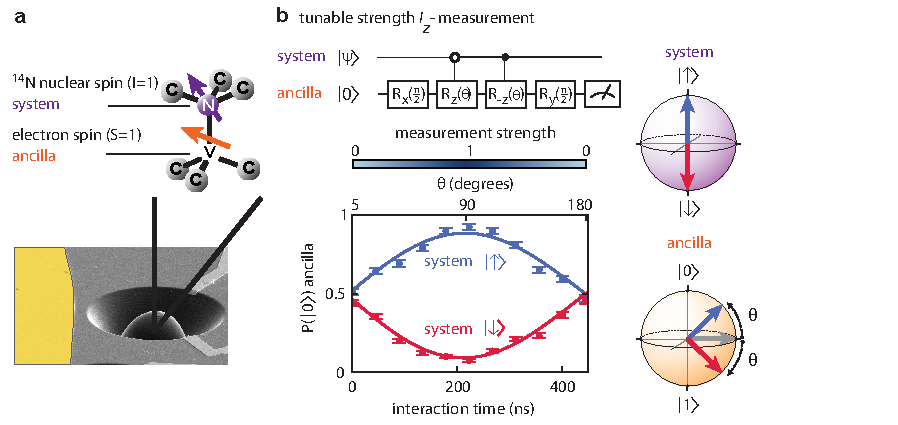
\includegraphics{fig1_twocolumns}
	\caption{\label{fig:amc-fig1} \textbf{Partial measurement of a spin qubit in diamond.} (a) The NV center is a natural two-qubit system where the system qubit is defined by the $^{14}N$ nuclear spin and the ancilla qubit is defined by the electron spin. A solid-immersion-lens is deterministically fabricated on top of the selected NV center to increase the photon collection efficiency. Control fields for single qubit rotations are generated by applying a current to the gold stripline (yellow).  (b) A tunable strength measurement is implemented by a Ramsey-type gate on the ancilla. We plot the probability to measure the state $\ket{0}$  for the ancilla, as a function of interaction time $\tau$, for two system input states $\ket{\downarrow}$ (red) and $\ket{\uparrow}$ (blue). The Bloch-spheres show the state of the system (purple) and ancilla (orange) after the entangling-gate for the different input states (red and blue vectors). The colour bar represents the measurement strength, proportional to $\sin{\theta}$, where $\theta=\frac{A \tau}{2}$. Blue corresponds to a projective measurement and white to no measurement. Solid lines are a  fit to the function $y_0 + e^{-( \frac{\tau}{T_2^*})^2} \cos{(A \tau + \delta)} $. From the phase offset $\delta$ we find the weakest measurement we can perform, corresponding to $\theta = 5^{\circ}$. This is limited by free evolution of the ancilla during the pulses.(see !!!TODO REFERENCE SOM!!!). Error bars depict 68 $\%$ confidence intervals. Sample size is 500 for each data point. }
\end{figure*}

We realize the variable-strength measurement by correlating the system qubit with the ancilla through a controlled-phase-type gate (Fig.\,\ref{fig:amc-fig1}b) that exploits the hyperfine interaction, which (neglecting small off-diagonal terms) has the form $\hat{H}_{hf}=A\hat{S}_{z}\hat{I}_{z}$ (with $A = 2 \pi \times 2.184 \pm 0.002$ MHz and $\hat{S}_{z}, \hat{I}_{z}$ the three-level Pauli z-operators for the electron, nuclear spin respectively).  During free evolution, the ancilla qubit precession is conditional on the state of the system qubit. We choose the rotating frame such that the ancilla rotates clockwise (anti-clockwise) around the z-axis if the system qubit is in $\ket{\uparrow}$ ($\ket{\downarrow}$) and vary the interaction time $\tau$. For $\tau = 0$, there is no correlation between the ancilla and the system, whereas for $\tau = \frac{\pi}{A}$, corresponding to the rotation angle $\theta = 90^{\circ}$, the two are maximally correlated. A subsequent rotation and projective readout of the ancilla then implements a measurement of the system qubit, with a measurement strength that can be accurately tuned by controlling the interaction time $\tau$. A mathematical derivation  can be found in the !!! TODO: REFERENCE TO SOM!!!

We investigate the measurement-induced backaction by preparing an initial state of the system ($\ket{\up},\ket{x}$ and $\ket{y}$) and performing a partial measurement with strength $\theta$, followed by state tomography (Fig.\,\ref{fig:amc-fig2}a). First, we neglect the outcome of the partial measurement, which is mathematically equivalent to taking the trace over the state of the ancilla qubit. In this case the backaction is equivalent to pure dephasing as can be seen by a measured reduction of the length of the Bloch vector (Fig.\,\ref{fig:amc-fig2}b). Next, we condition the tomography on the ancilla measurement yielding state $\ket{0}$ (Fig.\,\ref{fig:amc-fig2}c). We observe that for a weak measurement $(\theta = 5^{\circ})$, the system is almost unaffected, whereas for increasing measurement strength it receives a stronger kick towards $\ket{\uparrow} $(Fig.\,\ref{fig:amc-fig2}c). Crucially, we find that the length of the Bloch vector is preserved in this process, as expected for an initially pure state. This shows that the partial collapse is equivalent to a qubit rotation that is conditional on the measurement strength and outcome and on the initial state. By performing quantum process tomography, we find that both measurement processes agree well with the theoretical prediction (the process fidelities are 0.986 $\pm$ 0.004 and 0.94 $\pm$ 0.01 for the unconditional and conditional process, respectively; see !!!TO REFERENCE TO SOM!!!).


\begin{figure}
	\centering
	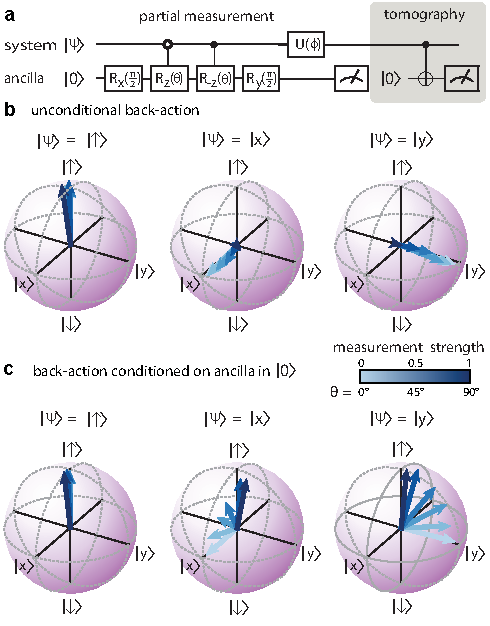
\includegraphics{fig2_partial_measurement_backaction}
	\caption{\label{fig:amc-fig2} \textbf{Measurement backaction for variable-strength measurement}. (a) We prepare an initial state  of the system ($\ket{\uparrow}$,  $\ket{x}$ and  $\ket{y}$), perform a partial measurement with strength $\theta$, and characterize the measurement backaction on the system by quantum state tomography. Quantum state tomography is implemented by an ancilla-assisted projective measurement, performed with the same protocol, setting $\tau = 229$ ns for $\theta = 90^{\circ}$. The nuclear spin basis rotation is performed with a $\frac{\pi}{2}$ radio-frequency pulse (along either $x$ or $y$). The basis rotation pulse for the tomography is applied before the readout of the ancilla, to avoid the dephasing induced by the state-characterization measurement (see main text). The data is corrected for errors in the readout and initialization of the system qubit, both of which are obtained from independent measurements (see !!! TODO REFERENCE SOM!!!). (b,c)  Measurement backaction for a partial measurement of increasing strength, independent of the measurement result for the ancilla qubit (b), or conditioned on the ancilla in  $\ket{0}$ (c). }
\end{figure}

\section{Generalized weak value}
By combining a partial measurement with post-selection on the outcome of a subsequent projective measurement, we can measure the generalized weak value $_{f} \langle I_{z} \rangle$ (conditioned average of contextual values \cite{Dressel_PRL_2010}, see !!TODO ADD REF TO SOM!!!) of the nuclear spin in the $z$-basis. In the limit of zero measurement strength ($\theta = 0^{\circ}$), this quantity approximates the weak value \cite{Aharonov_PRL_1988} $W = \frac{\bra{\psi_f} \hat{I}_z \ket{\psi_i}}{\bra{\psi_f} \psi_i \rangle}$ , where $ \psi_i (\psi_f )$ is the initial (final) state of the nucleus and from here we define $\hat{I}_z$ as the Pauli $z$-operator reduced to a two-level system with eigenvalues +1 and $-$1. By post-selecting only on the final states having small overlap with the initial state, $_{f} \langle I_{z} \rangle$ can be greatly amplified to values that lie outside the range of eigenvalues of the measured observable. As shown in Fig.\,\ref{fig:amc-fig3}, by sweeping the angle between the initial and final states we observe up to tenfold amplification ($_{f} \langle I_{z} \rangle = 10 \pm 3$) compared to the maximum eigenvalue of $I_{z}$ ($+1$). This amplification is the highest reported for a solid-state system to date\cite{Groen_PRL_2013}. As predicted \cite{Williams_PRL_2008}, we observe that values of  $_{f} \langle I_{z} \rangle$ lying outside of the range of eigenvalues of $I_{z}$ can be found for any finite measurement strength.

\begin{figure}
	\centering
	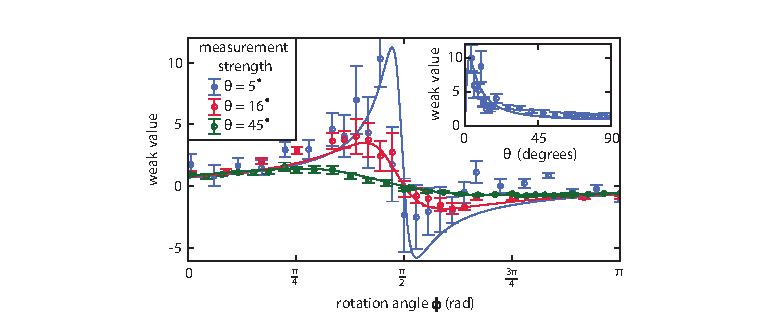
\includegraphics{fig3_weak_value}
	\caption{\label{fig:amc-fig3} \textbf{Generalized quantum weak value}. Measurement of a generalized weak value for the nuclear-spin qubit, performed by a partial measurement of strength $\theta$, followed by a strong measurement and post-selection of the state  $\ket{\downarrow}$, as a function of the basis rotation angle $\phi$ of the strong measurement (Fig.\,\ref{fig:amc-fig2}a). Solid lines are simulations using independently determined parameters. The asymmetry in the curve can be explained by asymmetric nuclear spin flips arising during ancilla initialisation by optical excitation of the forbidden transition of $E_{y}$ (see !!TODO REFERENCE SOM!!). Inset: the generalized weak values as a function of the strength $\theta$ of the partial measurement, setting the basis rotation angle of the strong measurement to the optimal value  $\phi = \frac{\pi}{2} - \theta$. All error bars depict 68 $\%$ confidence intervals. The sample size varies per data point because each data point has different post-selection criterion.}
\end{figure}

\section{QND-measurement of the ancilla qubit}
Using the partial measurements for measurement-based feedback requires reading out the ancilla without perturbing the system qubit. In our experiment the system qubit can dephase during ancilla readout both through a spin-flip of the electron in the course of optical excitation (Fig.\,\ref{fig:amc-fig4}b) and as a result of the difference in the effective nuclear g-factor in the electronic ground- and optically excited state~\cite{Jiang_PRL_2008}. Note that for the characterization of a single partial measurement (Fig.\,\ref{fig:amc-fig2}) we circumvent this dephasing by interchanging the measurement basis rotation and the ancilla readout; this interchange is not possible for real-time adaptive measurements.

\begin{figure*}
	\centering
	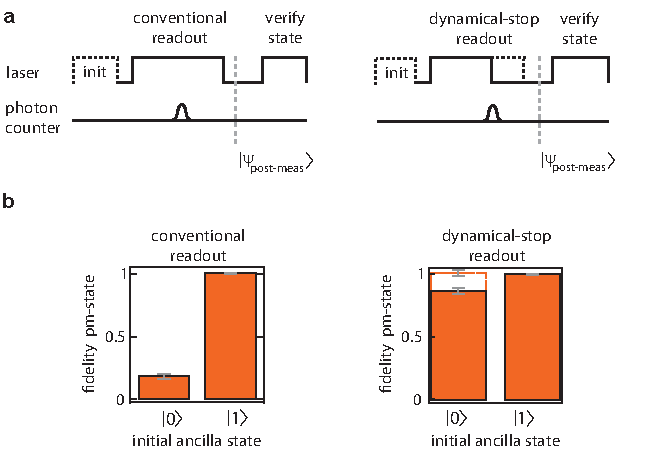
\includegraphics{fig4_qnd_electron}
	\caption{\label{fig:amc-fig4} \textbf{Quantum non-demolition measurement of the ancilla qubit} (a) The ancilla is initialized in $\ket{0}$ ($\ket{1}$) by optically pumping the $A_2$ ($E_y$) transition. The ancilla is then read out by exciting the $E_y$ transition for 100 $\mu$s (conventional readout), or until a photon was detected (dynamical-stop readout). Finally, we verify the post-measurement state with a conventional readout. (b) Fidelity of the post-measurement state of the ancilla for conventional readout (left graph) and dynamical-stop readout (right graph). Results are corrected for the infidelity in the final readout.  All error bars depict 68 $\%$ confidence intervals. Sample size per datapoint is 5000 }
\end{figure*}

To mitigate the nuclear dephasing during ancilla readout we reduce the ancilla spin-flip probability using a dynamical-stop readout technique. We partition the optical excitation time in short ($1~ \mu$s) intervals and we stop the excitation laser as soon as a photon is detected, or after a predetermined maximum readout time when no photon is detected (Fig.\,\ref{fig:amc-fig4}a). This reduces redundant excitations without compromising the readout fidelity. In Fig.\,\ref{fig:amc-fig4}b we show the correspondence between pre- and post-measurement states for the two eigenstates of the ancilla. For the state $\ket{0}$ the dynamical-stop readout increases the fidelity ($F = \bra{\psi_i}\rho_m \ket{\psi_i}$, where $\rho_m$ is the density matrix of the system after the ankle readout) from 0.18 $\pm$ 0.02 to 0.86 $\pm$ 0.02. The latter fidelity is solely limited by the cases where the spin flipped before a photon was detected: we find $F = 1.00 \pm 0.02$ for the cases in which a photon was detected. As expected, the fidelity is high ($F = 0.996 \pm 0.006$) for input state $\ket{1}$ as this state is unaffected by the excitation laser. The dynamical-stop technique thus implements a quantum non-demolition (QND) measurement of the ancilla electron spin with an average fidelity of 0.93 $\pm$ 0.01 for the post-measurement state.

The dynamical-stop readout of the ancilla significantly reduces the dephasing of the nuclear spin qubit during measurement as shown in Fig.\,\ref{fig:amc-fig5}. Starting with the nuclear spin in state $\ket{x} = \frac{\ket{0} + \ket{1}}{\sqrt{2}}$, a conventional readout of the ancilla completely dephases the nuclear spin, leading to a state fidelity with respect to $\ket{x}$ of 0.5. In contrast, the fidelity of the dynamical-stop readout saturates to 0.615 $\pm$ 0.002 (probably limited by changes in the effective g-factor of the nuclear spin). The dynamical-stop readout thus leaves the system in a coherent post-measurement state that can be used in a real-time feedback protocol. 

\begin{figure*}
	\centering
	\includegraphics{fig5_qnd_nuclear_spin}
	\caption{\label{fig:amc-fig5} \textbf{System qubit coherence during ancilla readout}. Coherence of the system qubit state after ancilla readout. For the dynamical-stop protocol we define the ancilla readout time as the predetermined maximum readout time. The graph shows the fidelity of the system with respect to $\ket{x}$ for conventional readout (red) and dynamical-stop readout (blue). The $z$-component of the system is unaffected as shown by the constant fidelity with respect to $\ket{\uparrow}$ (grey). All error bars depict 68 $\%$ confidence intervals. Sample size per datapoint is 2000 }
\end{figure*}

\section{Control by adaptive measurements}
Preserving coherence of the post-measurement state enables a proof-of-principle realization of measurement-only control, by implementing sequential measurements and tuning the strength of the second measurement in real time conditioned on the outcome of the first measurement (Fig.\,\ref{fig:amc-fig6}a). We choose as our target the creation of the state $\ket{\psi} = \cos{(\frac{\pi}{4}+\frac{\theta_1}{2})}\ket{\downarrow}+\cos{(\frac{\pi}{4}-\frac{\theta_1}{2})}\ket{\uparrow}$ from initial state $\ket{x}$ using only partial measurements of $\hat{I}_z$. The first measurement with strength $\theta_1$ will prepare either the desired state, or the state $\ket{\psi_{wrong}} =  \cos{(\frac{\pi}{4}-\frac{\theta_1}{2})}\ket{\downarrow}+\cos{(\frac{\pi}{4}+\frac{\theta_1}{2})}\ket{\uparrow}$ , each with probability 0.5. We adapt the strength of the second measurement $\theta_2$ according to the outcome of the first measurement: we set $\theta_2 = 0$ if the first measurement directly yielded the target state, but if the wrong outcome was obtained we set the measurement strength to

\begin{equation}
\theta_2 = \sin{^{-1}\left[2 \frac{\sin{\theta_1}}{1 + \sin{^2 \theta_1}}\right]},
\end{equation}

such that the second measurement will probabilistically rotate the qubit to the target state (see !!!TODO REF to sup!!!). The total success probability of this two-step protocol is  $p_{suc} = \frac{1}{2}(1 + \cos{\theta_1})$ and a successful event is heralded by the outcome of the ankle readout. In principle the protocol can be made fully deterministic~\cite{Ashhab_PhysRevA_2010} by incorporating a reset in the form of a projective measurement along the $x$-axis.

To find the improvement achieved by the feedback, we first compare the success probability of our adaptive measurement protocol to the success probability for a single measurement (Fig.\,\ref{fig:amc-fig6}b right panel). The success probability clearly increases with the adaptive protocol and is proportional to the readout fidelity of the $\ket{0}$ state of the ancilla, which is maximum for readout times  \textgreater~25~$\mu$s. The fidelity of the final state (Fig.\,\ref{fig:amc-fig6}b left panel) is limited by the remaining dephasing of the system during readout of the ancilla as shown in Fig.\,\ref{fig:amc-fig5}. This constitutes the trade-off between success probability and state fidelity. 

We show that the increase in success probability is non-trivial by comparing the final state fidelity with and without feedback (Fig.\,\ref{fig:amc-fig6}b left panel). In principle the success probability can be increased in the absence of feedback by accepting a certain number of false measurement outcomes at the cost of a reduced fidelity. We calculate the maximum fidelity that can be achieved in this way by performing only the first measurement and increasing the success probability to that of the adaptive protocol using post-selection (grey line in Fig.\,\ref{fig:amc-fig6}b, left panel). We find that the measured state fidelity in the adaptive protocol is above this bound (Fig.\,\ref{fig:amc-fig6}b, green area), which indicates that the adaptive measurement indeed successfully corrects the kickback from the first measurement, thus yielding a clear advantage over open-loop protocols.



We note that, in contrast to pioneering adaptive measurement experiments on photons that only used experimental runs in which a photon was detected at each measurement stage~\cite{Prevedel_Nature_2007}, our protocol is fully deterministic in the sense that the partial measurement always yields an answer. In particular, the data in Fig.\,\ref{fig:amc-fig6} includes all experimental runs and thus no post-selection is performed, as desired for future applications in metrology and quantum computing. 

The performance of the protocol can be further improved by increasing the ancilla readout fidelity (either by improving the collection efficiency or reducing spin-flip probability) and by further reducing the dephasing of the system during readout. A particularly promising route is to use nuclear spins farther away from the NV center (for example carbon-13 spins) that have much smaller hyperfine couplings~\cite{Zhao_NatureNano_2012,Taminiau_PRL_2012,Kolkowitz_PRL_2012} and are more robust against changes in the orbital state of the electron spin.

\begin{figure*}
	\centering
	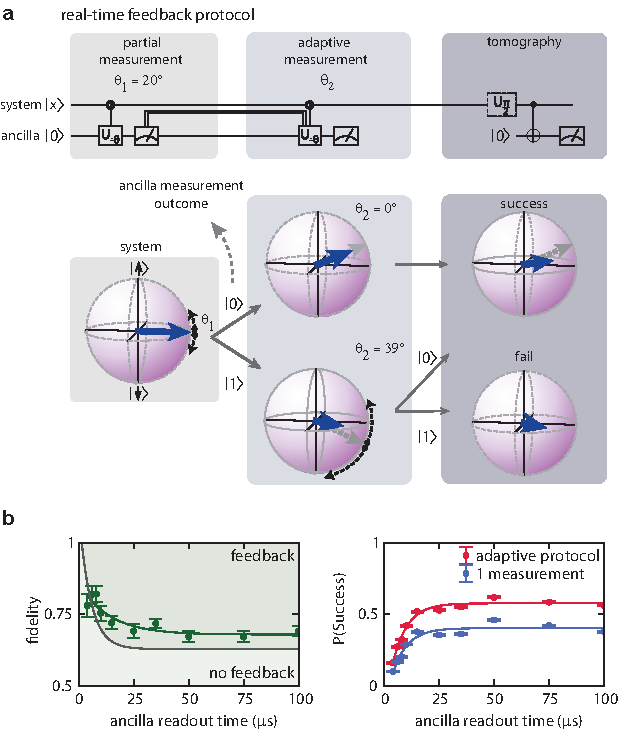
\includegraphics{fig6_adaptive_protocol}
	\caption{\label{fig:amc-fig6} \textbf{Manipulation of a nuclear spin state by sequential partial adaptive measurements with real-time feedback.} (a) Adaptive measurement protocol. The ancilla qubit is initialized in $\ket{0}$ and the system qubit is prepared in $\ket{x}$. The strength of the second measurement ($\theta_2$) is adjusted according to the outcome of the first measurement. The system is analysed by state tomography at each intermediate step. The result of the tomography is plotted on the bloch spheres (blue vector) and compared with the ideal case (grey vector). (b) Fidelity of the output state with respect to the target state as a function of ancilla readout time (dynamical-stop readout) with feedback (only the cases where the protocol heralds success). The grey line is obtained by performing one measurement and adding negative results to artificially increase the success probability to that of the adaptive protocol (red line in right panel). In the right panel we show the probability that the protocol heralds success for one measurement and for the adaptive protocol.  }
\end{figure*}

Our work is the first experimental exploration of a fundamental concept of control-free control \cite{Jordan_PRB_2006, Ashhab_PhysRevA_2010, Wiseman_NatureNV_2011} . Furthermore, the use of adaptive measurements as presented here can increase the performance of spin-based magnetometers \cite{Cappellaro_PhysRevA_2012, Higgins_Nature_2007}. Finally, our results can be combined with recently demonstrated methods for generating entanglement between separate nitrogen vacancy centre spins \cite{Bernien_Nature_2013, Dolde_NatPhys_2013}. Taken together, these techniques form the core capability required for one-way quantum computing, where quantum algorithms are executed by sequential adaptive measurements on a large entangled 'cluster' state \cite{Raussendorf_PRL_2001, Prevedel_Nature_2007}.

%In conclusion, we implemented sequential partial measurements and showed that by adjusting the measurement strength in real-time we can steer a quantum system towards a desired state. Our work is the first experimental exploration of a fundamental concept in the field of quantum measurement and control~\cite{Wiseman_NatureNV_2011} that may find application in systems where control fields are difficult to generate. Furthermore, the use of adaptive measurements as presented here can increase the performance of spin-based magnetometers~\cite{Cappellaro_PhysRevA_2012,Higgins_Nature_2007}. Finally, our results can be combined with recently demonstrated methods for generating entanglement between separate NV center spins~\cite{Bernien_Nature_2013,Dolde_NatPhys_2013}. Taken together, these techniques form the core capability required for one-way quantum computing, where quantum algorithms are executed by sequential adaptive measurements on a large entangled ‘cluster’ state~\cite{Raussendorf_PRL_2001,Prevedel_Nature_2007}.

\section{Methods}
We use a naturally-occurring nitrogen-vacancy center in high-purity type IIa CVD diamond, with a \textless 111\textgreater-crystal orientation obtained by cleaving and polishing a \textless100\textgreater -substrate. Experiments are performed in a bath cryostat, at the temperature of 4.2~K, with an applied magnetic field of 17~G. Working at low-temperature, we can perform efficient electron spin initialization (F~=~0.983~$\pm$~0.006) and single-shot readout (the fidelity is 0.853~$\pm$~0.005 for $m_S = 0$ and 0.986~$\pm$~0.002 for $m_S = -1$) by spin-resolved optical excitation~\cite{Robledo_Nature_2011}. Initialization of the nuclear spin is done by measurement~\cite{Robledo_Nature_2011}, with fidelity  0.95~$\pm$~0.02. Single-qubit operations can be performed with high accuracy using microwave (for the electron) and radio-frequency (for the nucleus) pulses applied to the gold stripline. Note that the single-qubit operations on the nucleus are only used for state preparation and tomography, but not in the feedback protocol. The dephasing time $T_2^*$ is (7.8~$\pm$~0.2)~ms for the nuclear spin and (1.35~$\pm$~0.03)~$\mu$s for the electron spin. 



\newpage
\bibliographystyle{../thesis}
\bibliography{amc}



%

\graphicspath{{./ch_adptv_msmnt_magnetometry/figures/}}


\chapter{ Optimized quantum sensing with a single electron spin
using real-time adaptive measurements}
\label{ch:AMM}


{\renewcommand{\thefootnote}{}\footnote{This chapter has been submitted to
    {\em Nature Nanotechnology} (2015).}}

\begin{center} 
    \vspace{-1cm} {C.~Bonato, M.S.~Blok, H.T. ~Dinani, D.W. ~Berry, M.L. ~Markham, D.J. ~Twitchen  and R.~Hanson} 
\end{center}


\vspace{-0.5cm} 
Quantum sensors based on single solid-state spins promise a unique combination of sensitivity and spatial resolution1-20. The key challenge in sensing is to achieve minimum estimation uncertainty within a given time and with a high dynamic range. Adaptive strategies have been proposed to achieve optimal performance but their implementation in solid-state systems has been hindered by the demanding experimental requirements. Here we realize adaptive d.c. sensing by combining single-shot readout of an electron spin in diamond with fast feedback. By adapting the spin readout basis in real time based on previous outcomes we demonstrate a sensitivity in Ramsey interferometry surpassing the standard measurement limit. Furthermore, we find by simulations and experiments that adaptive protocols offer a distinctive advantage over the best-known non-adaptive protocols when overhead and limited estimation time are taken into account. Using an optimized adaptive protocol we achieve a magnetic field sensitivity of $6.1\pm 1.7$ nT Hz$^{-\frac{1}{2}}$ over a wide range of 1.78 mT. These results open up a new class of experiments for solid-state sensors in which real-time knowledge of the measurement history is exploited to obtain optimal performance.


\clearpage

\section{Introduction}
Quantum sensors have the potential to achieve unprecedented sensitivity by exploiting control over individual quantum systems1,2. As a prominent example, sensors based on single electron spins associated with Nitrogen-Vacancy (NV) centers in diamond capitalize on the spin?s quantum coherence and the high spatial resolution resulting from the atomic-like electronic wave function3,4. Pioneering experiments have already demonstrated single-spin sensing of magnetic fields5-7, electric fields8, temperatures9,10 and strain11. NV sensors may therefore have a revolutionary impact on biology12-15, nanotechnology16-18 and material science19,20. 

A spin-based magnetometer can sense a d.c. magnetic field \textit{B} through the Zeeman shift $E_z=\hbar \gamma B = \hbar 2 \pi f_B$ ($\gamma$ is the gyromagnetic ratio and $f_B$ the Larmor frequency) between two spin levels $\ket{0}$ and $\ket{1}$. In a Ramsey interferometry experiment, a superposition state  $\frac{1}{\sqrt{2}}$($\ket{0}$ + $\ket{1}$), prepared by a $\pi$/2 pulse, will evolve to $\frac{1}{\sqrt{2}}$($\ket{0}$ + $e^{i\phi}\ket{1}$)   over a sensing time \textit{t}. The phase $\phi = 2 \pi f_B t$ can be measured by reading out the spin in a suitable basis, by adjusting the phase $\vartheta$ of a second $\pi$/2 pulse.


For a Ramsey experiment that is repeated with constant sensing time \textit{t} the uncertainty $\sigma_{f_B}$ decreases with the total sensing time \textit{T} as 1/(2 $\pi \sqrt{tT}$) (standard measurement sensitivity, SMS).  However, the field range also decreases with \textit{t} because the signal is periodic, creating ambiguity whenever $|2\pi f_B t| > \pi $. This results in a dynamic range bounded as  $f_{B,max}$/$\sigma_{f_B}  \le \pi \sqrt{T/t}$.  Recently, it was discovered that the use of multiple sensing times within an estimation sequence can yield a scaling of $\sigma_{f_B}$ as 1/\textit{T}, resulting in a vastly improved dynamic range: $f_{B,max}$/ $\sigma_{f_B} \le  \pi T $/$ \tau_{min}$, where $\tau_{min}$ is the shortest sensing time used. A major open question is whether adaptive protocols, in which the readout basis is optimized in real time based on previous outcomes, can outperform non-adaptive protocols. While scaling beating the standard measurement limit has been reported with non-adaptive protocols22,23, feedback techniques have only recently been demonstrated for solid-state quantum systems24-26 and adaptive sensing protocols have so far remained out of reach.


Here we implement adaptive d.c. sensing with a single-electron spin magnetometer in diamond by exploiting high-fidelity single-shot readout and fast feedback electronics (Fig.\,\ref{fig:amm-fig1}a). We demonstrate a sensitivity beyond the standard measurement limit over a large field range. Furthermore, we investigate through experiments and simulations the performance of different adaptive protocols and compare these to the best known non-adaptive protocol. Although the non-adaptive protocol improves on the standard measurement limit for sequences with many detections we find that the adaptive protocols perform better when overhead time for initialization and readout is taken into account. In particular, the adaptive protocols require shorter sequences to reach the same sensitivity, thus allowing for sensing of signals that fluctuate on shorter timescales.

\begin{figure*}
	\centering
	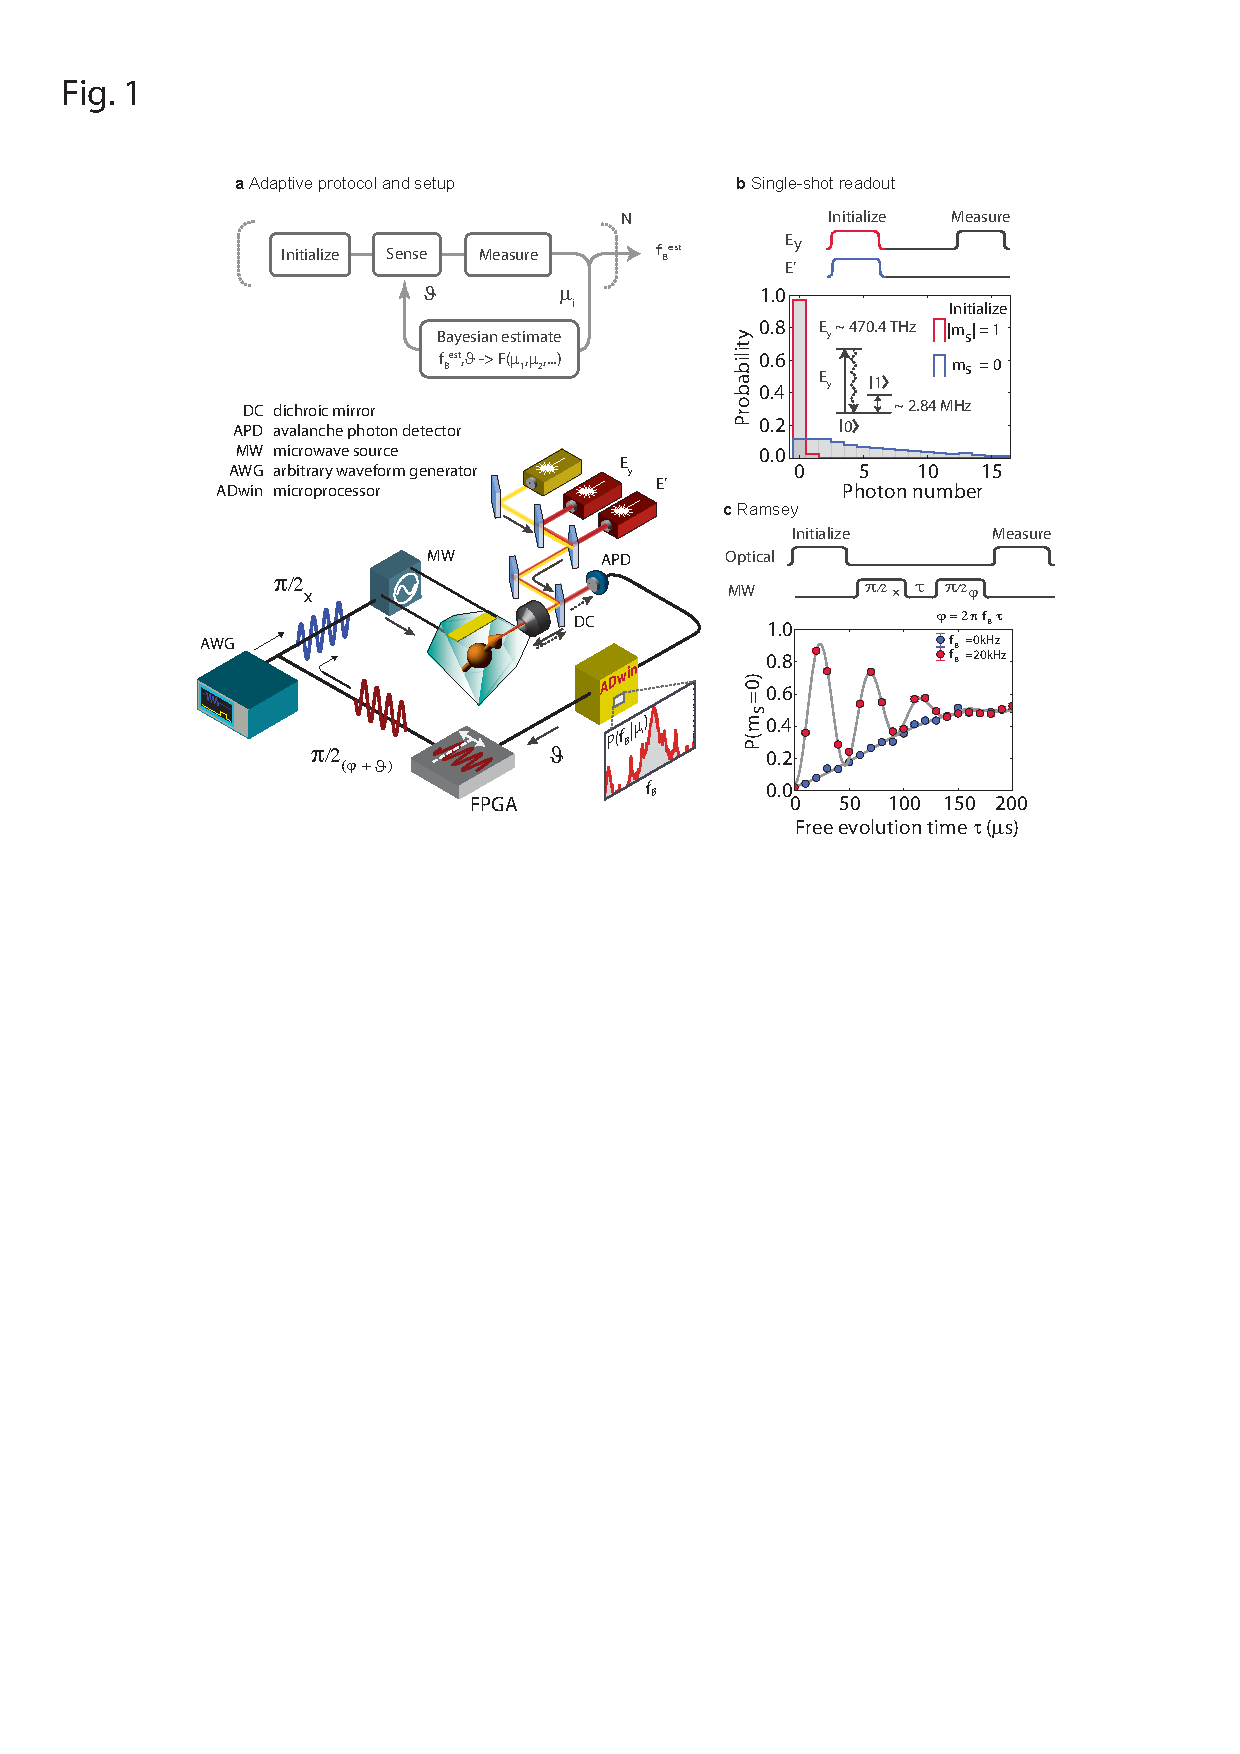
\includegraphics{Fig_1}
	\caption{\label{fig:amm-fig1} \textbf{Experiment concept and apparatus.} (a) The adaptive frequency estimation protocol consists of a sequence of initialization, sensing, measurement operations. After each measurement run, the outcome $\mu$ is used to update the estimate of the frequency $f_B$, which is then used to optimize the sensing parameters for the following run. Experimentally, the frequency estimation and adaptive calculation of the phase are performed in real-time by a microprocessor. (b) The experiment is performed using the states $\ket{0} = \ket{m_s = 0}$,$\ket{1} = \ket{m_s = -1}$ of the  electronic spin of a NV centre in diamond. The electronic spin is readout by resonant optical excitation and photon counting27: detection of luminescence photons corresponds to detection of the $\ket{0}$ state. We plot the probability of detecting a photon after initializing either in $\ket{0}$ or $\ket{1}$. The readout fidelities for the states $\ket{0}$ (outcome 0) and $\ket{1}$  (outcome 1) are $F_0 = 0.88 \pm 0.02$, $F_1 = 0.98 \pm 0.02$, respectively. (c) Each measurement run consists of a Ramsey experiment, in which the phase accumulated over time by a spin superposition during free evolution is measured. The measurement basis rotation is controlled by the phase $\vartheta$ of the final $\pi$/2-pulse. From the measured phase, we can extract the frequency $f_B$, corresponding to an energy shift between the levels $\ket{0}$ and $\ket{1}$ given by an external field (magnetic field, temperature, strain…). Here, to test the performance of different protocols, we set $f_B$ as an artificial detuning, set by the microprocessor by adding $\phi = 2 \pi f_B t$ to the phase $\vartheta$ (Supplementary Figure !!!TODO ADD REF!!!!!).}
\end{figure*}

Our magnetometer employs two spin levels of a single NV center electron in isotopically purified diamond (0.01 \% $^{13}C$). We exploit resonant spin-selective optical excitation, at a temperature of 8 K, for high-fidelity initialization and single-shot readout!!!TODO ADD REF!! (Fig.\,\ref{fig:amm-fig1}b). Microwave pulses, applied via an on-chip stripline, coherently control the electron spin state. From Ramsey experiments, we measure a spin dephasing time of $T_2^* = (96 \pm 2) \mu$s (Fig.\,\ref{fig:amm-fig1}c). In order to characterize the performance of different sensing protocols in a controlled setting, the effect of the external field is implemented as an artificial frequency detuning, by adding $\phi = 2 \pi f_B t$ to the phase $\vartheta$  of the final $\pi$/2-pulse. To achieve high sensitivity in a wide field range we use an estimation sequence consisting of \textit{N} different sensing times21-23,28, varying as $\tau_n = 2^{(N-n)} \tau_{min}$ ( \textit{n} = 1..\textit{N}). The value of $\tau_{min}$ sets the range; we take $\tau_{min}$ = 20 ns, corresponding to a range |$f_B$| < 25  MHz, equivalent to |\textit{B}| < 0.89 mT for $\gamma = 2 \pi \times 28$ MHz mT$^{-1}$.

The key idea of adaptive magnetometry is that for each Ramsey experiment the measurement basis is chosen based on the previous measurement outcomes such that the uncertainty in the frequency estimation is minimized (Fig.\,\ref{fig:amm-fig1}a). After every Ramsey experiment, the outcome is used to update a frequency probability distribution $P(f_B)$ according to Bayes’ rule, taking measured values for detection fidelity and coherence time into account (Methods). The current estimate of $P(f_B)$ is then used to calculate the phase $\vartheta$ of the final $\pi$/2-pulse which allows for best discrimination between different possible magnetic field values in the next Ramsey experiment28. In our experiment, this process is realized by a microprocessor, which receives the measurement outcome, performs the Bayesian estimate, calculates the  phase $\vartheta$ and subsequently sends a digital signal to a field-programmable gate array (FPGA) to adjust the phase of the final $\pi$/2-pulse accordingly (Fig.\,\ref{fig:amm-fig1}a).

To reduce the undesired effects of quantum projection noise and imperfect readout fidelity we perform $M_n$ Ramsey experiments21 for each sensing time $\tau_n$, with  $M_n = G + F (n-1)$. Here \textit{G} and \textit{F} can be chosen to optimize the performance of the protocol. For the short sensing times (large \textit{n}), corresponding to the measurements that make the largest distinction in frequency (and where an error is therefore most detrimental), we  perform the most Ramsey experiments. We will compare several protocols that differ in the strategy of adaptive phase choice. As a first example, we consider a protocol where the phase $\vartheta$ is adjusted each time the sensing time is changed; we name this “limited-adaptive” protocol. 

\begin{figure*}
	\centering
	\includegraphics{Fig_2}
	\caption{\label{fig:amm-fig2} \textbf{.}}
\end{figure*}

An example of the working principles of the limited-adaptive protocol is illustrated in Fig.\,\ref{fig:amm-fig2}, for an estimation sequence comprising $N = 3$ sensing times and one measurement per sensing time (\textit{G} = 1, \textit{F} = 0). We start with no information over $f_B$, corresponding to a uniform probability density $P(f_B )$ (solid black line).  For the first Ramsey experiment, the sensing time is set to $4 \tau_{min}$. $P(f_B)$ is updated depending on the measurement outcome. For example, the outcome 1 indicates maximum probability for the values $f_B = \pm 6.25, \pm 18.75$ MHz, and minimum probability for $f_B = 0, \pm 12.5, \pm 25$ MHz. This indeterminacy in the estimation originates from the fact that, for this sensing time, the acquired phase spans the range [-4$\pi$, 4$\pi$], wrapping multiple times around the [-$\pi$, $\pi$] interval. The sensing time is then decreased to $2 \tau_{min}$. Given the current $P(f_B)$ for outcome 1 (black curve), the filter functions that would be applied to $P(f_B)$ after the Bayesian update for detection outcomes 0 and 1 are represented, respectively, by the light red and blue areas. For $\vartheta = - /pi$/2, maximum distinguishability is ensured: outcome 0 would select the peaks around $f_B$ = -6.25, +18.75 MHz, while outcome 1 would select the peaks around $f_B$ = -18.75, +6.25 MHz. The same process is then repeated, decreasing the sensing time to  $\tau_{min}$. The remaining uncertainty, corresponding to the width of the resulting peak in $P(f_B)$, is set by the longest sensing time $4 \tau_{min}$. 

\begin{figure*}
	\centering
	\includegraphics{Fig_3}
	\caption{\label{fig:amm-fig3} \textbf{.}}
\end{figure*}

Figure \,\ref{fig:amm-fig3}b shows the probability density yielded by experimental runs of the limited-adaptive protocol with different numbers of sensing times \textit{N} = 1,3,5,7,9. Here,  $f_B$ = 2 MHz, and each estimation sequence is repeated 101 times, with \textit{G} = 5, \textit{F} = 7. For increasing \textit{N}, the width of the distribution becomes more narrowly peaked around the expected value of 2 MHz, while the wings of distribution are strongly suppressed. 

To verify that the protocol works over a large dynamic range, we measure the uncertainty as a function of detuning $f_B$. To account for the periodic nature of phase we use the Holevo variance $V_H = (|<\exp^{i2 \pi f_B^{est} \tau_{min}}>|)^2 - 1$ as a measure of the uncertainty. We estimate  $f_B^{est}$ by taking the mean of the probability density $P(f_B)$ resulting from a single run of the protocol. A fixed initial phase ($\vartheta$ = 0 in our experiments) results in a specific dependence of the variance on the magnetic field. For example, for \textit{N} = 2, only four measurement outcomes are possible $\{$ 00, 01, 10, 11 $\}$, corresponding to $f_B$ = 0, -25, -12.5, +12.5 MHz, respectively. These specific detunings can be measured with the highest accuracy since they correspond to measurements of an eigenstate of our quantum sensor at the end of the Ramsey experiment, while for other frequencies larger statistical fluctuations will be found due to spin projection noise. Figure \,\ref{fig:amm-fig3}c shows $V_H$ as a function of detuning for the parameters \textit{G} = 5, \textit{F} = 7. Both the experimental data (dots) and the numerical simulation (solid lines) confirm the expected periodic behavior.

We now use our adaptive sensing toolbox to compare different sensing protocols by investigating the scaling of $\eta^2 = V_H T$, averaged over different detunings, as a function of the total sensing time \textit{T}. First, we will ignore the overhead time due to spin initialization and readout. 

We compare the limited-adaptive protocol to the best known non-adaptive protocol and to an optimized adaptive protocol. In the non-adaptive protocol 21-23, the readout phase for the $m^{th}$ Ramsey experiment is always set to $\vartheta_{n,m} = \frac{m\pi}{M_n}$  ( \textit{m} = 1..$M_n$). In the optimized adaptive protocol29,30, the phase $\vartheta$ is updated before each Ramsey and, additionally, a phase $\vartheta_{n,m}^{incr}$ that depends only on the current values of \textit{n},\textit{m} and the last measurement outcome $\mu_{n,m}$, is added. This additional $\vartheta_{n,m}^{incr}$ is determined by a numerical minimization of the Holevo variance, via swarm-optimization techniques, taking experimental parameters into account. A detailed description of all protocols is reported in Supplementary Tables !! TO DO ADD REF!!!.

We plot experimental data for the sensitivity scaling for the three protocols in Fig.\,\ref{fig:amm-fig4}a alongside simulations using known experimental parameters. In these graph, the SMS limit corresponds to a constant $V_H T$; any scaling behavior with a negative slope thus improves beyond the SMS.

\begin{figure*}
	\centering
	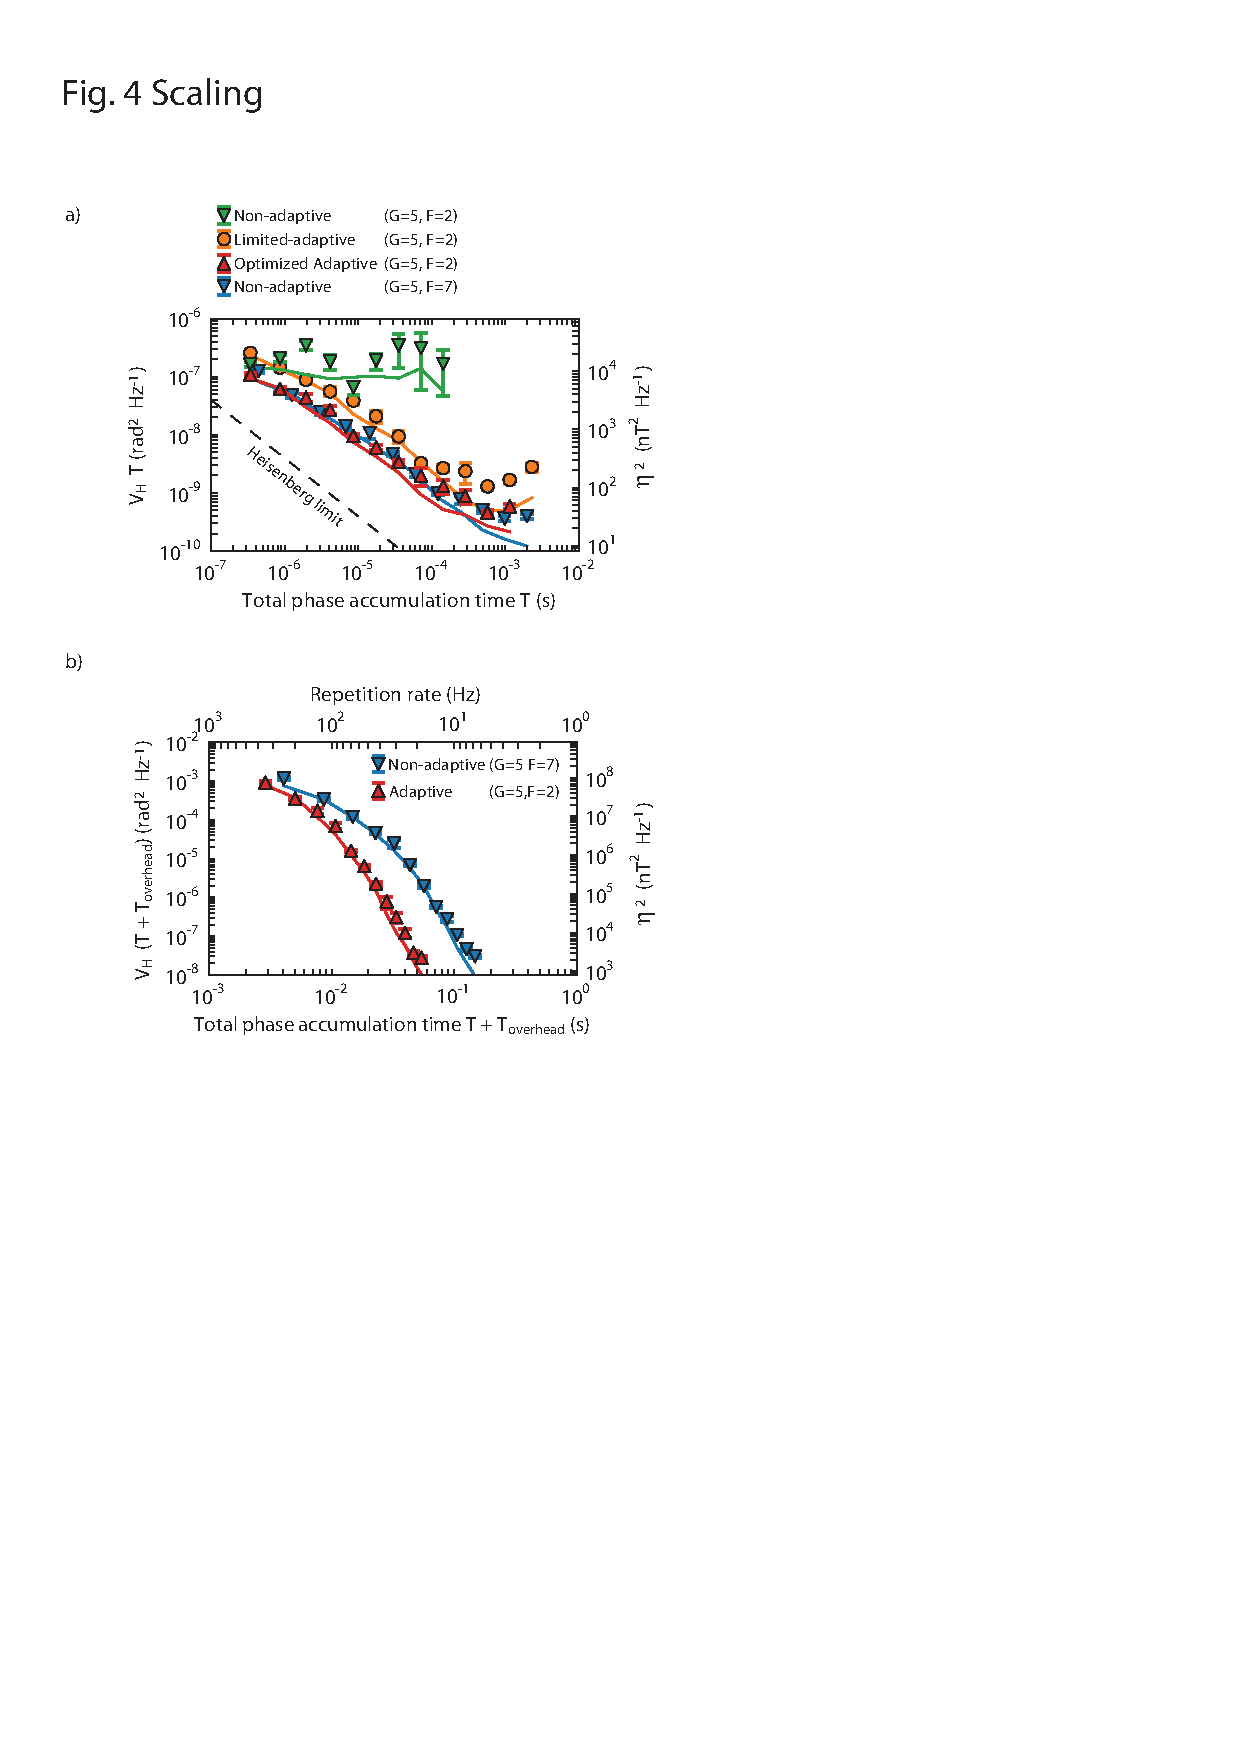
\includegraphics{Fig_4}
	\caption{\label{fig:amm-fig4} \textbf{.}}
\end{figure*}


We observe that, for the setting (\textit{G} = 5, \textit{F} = 2), the non-adaptive protocol reaches only the SMS limit, while both adaptive protocols yield $V_H T$ scaling close to 1/\textit{T}. When the number of measurements per interaction time is increased to (\textit{G} = 5, \textit{F} = 7) the non-adaptive protocol also shows sub-SMS scaling (Fig.\,\ref{fig:amm-fig4}a, blue line). We find this behavior to be quite general: both adaptive and non-adaptive protocols can reach 1/\textit{T} scaling, but the adaptive protocols require fewer measurements (Supplementary Figures !!TODO: ADD REF!!!). By comparing the best non-adaptive and the best adaptive protocol, we find that they reach the same sensitivity of (6.1 $\pm$ 1.7) nT Hz$^{-\frac{1}{2}}$ when the longest sensing time reaches $T_2^*$. The non-adaptive protocol however, requires significantly more measurements (611) than the adaptive protocol (221).


The advantage of adaptive measurements becomes clear when the initialization and readout times (overhead) are taken into account (Fig \,\ref{fig:amm-fig4}b). Since the time required to compute the controlled phase is similar to the initialization time, the two operations can be performed simultaneously, with no additional overhead required by the adaptive protocol (Methods). While the two best protocols still achieve similar minimum sensitivities, the optimized adaptive protocol requires significantly less measurement time. At any fixed measurement time, the adaptive protocol estimates the magnetic field more accurately, allowing a higher repetition rate for the estimation sequences. This is advantageous in the realistic situation that the magnetic field to be estimated is not static: in this case, the estimation time is required to be shorter than the timescale of the fluctuations. Our data shows that at an estimation repetition rate of 20 Hz, the non-adaptive protocol can estimate a magnetic field with an sensitivity $\eta$ = (749 $\pm$ 35) nT Hz$^{-\frac{1}{2}}$, while the optimized-adaptive protocol yields $\eta$ = (47 $\pm$ 2) nT Hz$^{-\frac{1}{2}}$.

While the record sensitivity reported here is enabled by single-shot spin readout at low temperature, adaptive techniques can prove valuable also in experiments at room temperature23 where spin-dependent luminescence intensity under off-resonant excitation is typically used to measure the electronic spin. By averaging the signal over multiple repetitions an arbitrarily high readout fidelity can be achieved (\textit{F} = 0.99 for 50,000 repetitions23). Interestingly, we find that the benefits given by adaptive techniques persist also in case of lower readout fidelities and that the combination of adaptive techniques and optimization of the number of readout repetitions yields a significant improvement (Supplementary Figure !!!TODO: ADD REF!!!).

In conclusion, by combining high-fidelity single-shot readout at low temperature with a single electron spin sensor and fast electronics, we achieve an unprecedented d.c. sensitivity of (6.1 $\pm$ 1.7) nT Hz$^{-\frac{1}{2}}$ with a repetition rate of 20 Hz. Another relevant figure of merit for sensors is the ratio between the range and the sensitivity; the best value found in this work ($B_{max}$/$\eta \sim 1.5 \cdot 10^5 $Hz$^{\frac{1}{2}}$) improves on previous experiments by two orders of magnitude22,23. Furthermore, we found that the best known adaptive protocol outperforms the best known non-adaptive protocol when overhead is taken into account. These insights can be extended to other quantum sensors and to the detection of different physical quantities such as temperature and electric fields. A remaining open question is whether this adaptive protocol is optimal; perhaps further improvements are possible by taking into account the full measurement history. In a more general picture, the adaptive sensing toolbox demonstrated in this work will enable exploration of the ultimate limits of quantum metrology and may lead to practical sensing devices combining high spatial resolution, sensitivity, dynamic range and repetition rate.



\section{Methods}
M
\section{Acknowledgements}
Bla

%\bibliography{adptv_msmnt_cntrl}

\graphicspath{{./ch_LDE/figures/}}

\chapter[Heralded entanglement and unconditional teleportation between solid-state qubits separated by three metres]{Heralded entanglement and unconditional teleportation between solid-state qubits separated by three metres}
\label{ch:LDE}

\begin{center} 
    \vspace{-1cm} {H.~Bernien, W.~Pfaff, B.~Hensen,  M.S.~Blok, T.H.~Taminiau, S.B.~van Dam, G.~Koolstra, L.~Robledo, M.J. ~Tiggelman, R.N. ~Schouten, M.~Markham, D.J.~Twitchen, L.~Childress, and R.~Hanson} 
\end{center}

{\renewcommand{\thefootnote}{}\footnote{The results in this chapter have been published in
    {\em Nature} \textbf{497}, 86 (2013) and {\em Science} \textbf{345}, 532 (2014).}}

\vspace{-0.5cm} 
Quantum entanglement between spatially separated objects is a unique resource for quantum information processing and communication. Entangled qubits can be used to establish private information or implement quantum logical gates~\cite{Nielsen__2000,Raussendorf_Phys.Rev.Lett._2001}. Such capabilities are particularly useful when the entangled qubits are spatially separated~\cite{Moehring_Nature_2007,Ritter_Nature_2012,Hofmann_Science_2012}, opening the opportunity to create highly connected quantum networks~\cite{Kimble_Nature_2008} or extend quantum cryptography to long distances~\cite{Duan_Nature_2001,Childress_Phys.Rev.Lett._2006}. Here we present two key experiments towards the realisation of long-distance quantum networks with solid-state quantum registers. Firstly, we have entangled two electron spin qubits in diamond that are separated by a three-metre distance. Our robust entangling protocol is based on local creation of spin-photon entanglement and a subsequent joint measurement of the photons to herald spin-spin entanglement. The resulting shared Bell-pair between the two nodes then enables the unconditional teleportation of a single nuclear spin state by combining a deterministic Bell-state measurement with real-time feed-forward. These results establish diamond spin qubits as a prime candidate for the realization of quantum networks for quantum communication and network-based quantum computing

% Detection of the photons heralds the projection of the spin qubits onto an entangled state. We verify the resulting non-local quantum correlations by performing single-shot readout~\cite{Robledo2011} on the qubits in different bases. The long-distance entanglement reported here can be combined with recently achieved initialisation, readout and entanglement operations~\cite{Robledo2011,Neumann2010a,Neumann2008,Maurer2012,Pfaff2012} on local long-lived nuclear spin registers, enabling deterministic long-distance teleportation, quantum repeaters and extended quantum networks.

\clearpage

\section{Introduction}

A quantum network can be constructed by using entanglement to connect local processing nodes, each containing a register of well-controlled and long-lived qubits~\cite{Kimble_Nature_2008}. Solids are an attractive platform for such registers, as the use of nano-fabrication and material design may enable well-controlled and scalable qubit systems~\cite{Ladd_Nature_2010}. The potential impact of quantum networks on science and technology has recently spurred research efforts towards generating entangled states of distant solid-state qubits~\cite{Togan_Nature_2010,Gao_Nature_2012,DeGreve_Nature_2012,Bernien_Phys.Rev.Lett._2012,Sipahigil_Phys.Rev.Lett._2012,Patel_NatPhoton_2010,Flagg_Phys.Rev.Lett._2010}.

A prime candidate for a solid-state quantum register is the nitrogen-vacancy (NV) defect centre in diamond. The NV centre combines a long-lived electronic spin (S=1) with a robust optical interface, enabling measurement and high-fidelity control of the spin qubit~\cite{Togan_Nature_2010,Fuchs_Science_2009,Lange_Science_2010,vanderSar_Nature_2012}. Furthermore, the NV electron spin can be used to access and manipulate nearby nuclear spins~\cite{Robledo_Nature_2011,Neumann_Science_2010,Neumann_Science_2008,Maurer_Science_2012,Pfaff_NatPhys_2013}, thereby forming a multi-qubit register. To use such registers in a quantum network requires a mechanism to coherently connect remote NV centres.

!! make more general to include teleportation!! Here we demonstrate the generation of entanglement between NV centre spin qubits in distant setups. We achieve this by combining recently established spin initialisation and single-shot readout techniques~\cite{Robledo_Nature_2011} with efficient resonant optical detection and feedback-based control over the optical transitions, all in a single experiment and executed with high fidelity. These results put solid-state qubits on par with trapped atomic qubits~\cite{Moehring_Nature_2007,Ritter_Nature_2012,Hofmann_Science_2012} as highly promising candidates for implementing quantum networks.

Our experiment makes use of two NV spin qubits located in independent low-temperature setups separated by 3 metres (Fig.\,\ref{fig:LDE-fig1-setup}). We encode the qubit basis states $\ket{\up}$ and $\ket{\down}$ in the NV spin sub-levels $\mszero$ and $\msmone$, respectively. Each qubit can be independently read out by detecting spin-dependent fluorescence in the NV phonon side band (non-resonant detection)~\cite{Robledo_Nature_2011}. The qubits are individually controlled with microwave pulses applied to on-chip strip-lines~\cite{Lange_Science_2010}. Quantum states encoded in the qubits are extremely long-lived: using dynamical decoupling techniques~\cite{Lange_Science_2010} we obtain a coherence time exceeding 10$\,$ms (Fig.\,\ref{fig:LDE-fig1-DD}), the longest coherence time measured to date for a single electron spin in a solid.

\begin{figure}[tp]
	\centering
	\includegraphics{fig1_entanglement_setup}
	\caption{\label{fig:LDE-fig1-setup} \textbf{Experimental setup.} a Each nitrogen vacancy (NV) centre resides in a synthetic ultra-pure diamond oriented in the $\langle 111\rangle$ direction. The two diamonds are located in two independent low-temperature confocal microscope setups separated by 3 metres. The NV centres can be individually excited resonantly by a red laser and off-resonantly by a green laser. The emission (dashed arrows) is spectrally separated into an off-resonant part (phonon side band, PSB) and a resonant part (zero-phonon line, ZPL). The PSB emission is used for independent single-shot readout of the spin qubits~\cite{Robledo_Nature_2011}. The ZPL photons from the two NV centres are overlapped on a fiber-coupled beamsplitter. Microwave pulses for spin control are applied via on-chip microwave strip-lines. An applied magnetic field of 17.5\,G splits the $\mspmone$ levels in energy. The optical frequencies of NV~B are tuned by a d.c. electric field applied to the gate electrodes ((b) scanning electron microscope image of a similar device). To enhance the collection efficiency, solid immersion lenses have been milled around the two NV centres~\cite{Robledo_Nature_2011}. }
\end{figure}

	
\section{Heralded entanglement}\label{sec:HE}

We generate and herald entanglement between these distant qubits by detecting the resonance fluorescence of the NV centres. The specific entanglement protocol we employ is based on the proposal of S. Barrett and P. Kok~\cite{Barrett_Nature_2004}, and is schematically drawn in figure~\ref{fig:LDE-fig1-protocol}. Both centres NV~A and NV~B are initially prepared in a superposition $1/\sqrt{2}(\ket{\up}+\ket{\down})$. Next, each NV centre is excited by a short laser pulse that is resonant with the $\ket{\up}$ to $\ket{e}$ transition, where $\ket{e}$ is an optically excited state with the same spin projection as $\ket{\up}$. Spontaneous emission locally entangles the qubit and photon number, leaving each setup in the state $1/\sqrt{2}(\ket{\uparrow 1}+\ket{\downarrow 0})$, where 1 (0) denotes the presence (absence) of an emitted photon; the joint qubit-photon state of both setups is then described by $1/2(\ket{\uparrow_\text{A}\uparrow_\text{B}}\ket{1_\text{A}1_\text{B}}+\ket{\downarrow_\text{A}\downarrow_\text{B}}\ket{0_\text{A}0_\text{B}}+\ket{\uparrow_\text{A}\downarrow_\text{B}}\ket{1_\text{A}0_\text{B}}+\ket{\downarrow_\text{A}\uparrow_\text{B}}\ket{0_\text{A}1_\text{B}})$. The two photon modes, A and B, are directed to the input ports of a beamsplitter (see Fig.~\ref{fig:LDE-fig1-setup}a), so that fluorescence observed in an output port could have originated from either NV centre. If the photons emitted by the two NV centres are indistinguishable, detection of precisely one photon on an output port would correspond to measuring the photon state $\ket{1_\text{A}0_\text{B}}\pm e^{-i\varphi}\ket{0_\text{A}1_\text{B}}$ (where $\varphi$ is a phase that depends on the optical path length). Such a detection event would thereby project the qubits onto a maximally entangled state $\ket{\psi}=1/\sqrt{2}(\ket{\uparrow_\text{A}\downarrow_\text{B}}\pm e^{-i\varphi}\ket{\downarrow_\text{A}\uparrow_\text{B}})$.
\begin{figure}[tp]
	\centering
	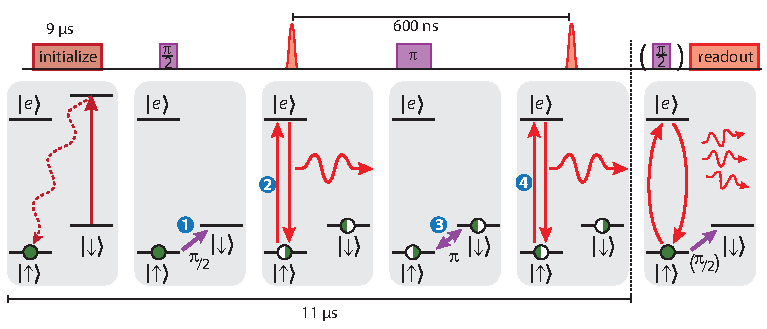
\includegraphics{fig1_entanglement_protocol}
	\caption{\label{fig:LDE-fig1-protocol} \textbf{Protocol.} Entanglement protocol (details in main text), illustrating the pulse sequence applied simultaneously to both NV centres. Both NV centres are initially prepared in a superposition $1/\sqrt{2}(\ket{\up}+\ket{\down})$. A short $2\,$ns spin-selective resonant laser pulse creates spin-photon entanglement $1/\sqrt{2}(\ket{\uparrow 1}+\ket{\downarrow 0})$. The photons are overlapped on the beamsplitter and detected in the two output ports. Both spins are then flipped, and the NV centres are excited a second time. The detection of one photon in each excitation round heralds the entanglement and triggers individual spin readout.}
\end{figure}

Any realistic experiment, however, suffers from photon loss and imperfect detector efficiency; detection of a single photon is thus also consistent with creation of the state $\uu$. To eliminate this possibility, both qubits are flipped and optically excited for a second time. Since $\uu$ is flipped to $\dd$, no photons are emitted in the second round for this state. In contrast, the states $\ket{\psi}$ will again yield a single photon. Detection of a photon in both rounds thus heralds the generation of an entangled state. The second round not only renders the protocol robust against photon loss, but it also changes $\varphi$ into a global phase, making the protocol insensitive to the optical path length difference~\cite{Barrett_Phys.Rev.A_2005} (see Supporting Material). Furthermore, flipping the qubits provides a refocusing mechanism that counteracts spin dephasing during entanglement generation. The final state is one of two Bell states $\ket{\psi^\pm}=1/\sqrt{2}(\ket{\uparrow_\text{A}\downarrow_\text{B}}\pm\ket{\downarrow_\text{A}\uparrow_\text{B}})$, with the sign depending on whether the same detector ($+$), or different detectors ($-$) clicked in the two rounds.

\subsection{Implementation}

A key challenge for generating remote entanglement with solid-state qubits is obtaining a large flux of indistinguishable photons, in part because local strain in the host lattice can induce large variations in photon frequency. The optical excitation spectra of the NV centres (Fig.~\ref{fig:LDE-fig2}a) display sharp spin-selective transitions. Here we use the $E_\text{y}$ transition (spin projection $\mszero$) in the entangling protocol and for qubit readout; we use the $A_1$ transition for fast optical pumping into $\ket{\up}$~\cite{Robledo_Nature_2011}. Due to different strain in the two diamonds, the frequencies of the $E_\text{y}$ transitions differ by 3.5$\,$GHz, more than 100 line-widths. By applying a voltage to an on-chip electrode (Fig.~\ref{fig:LDE-fig1-setup}b) we tune the optical transition frequencies of one centre (NV~B) through the d.c. Stark effect~\cite{Bernien_Phys.Rev.Lett._2012,Bassett_Phys.Rev.Lett._2011} and bring the $E_\text{y}$ transitions of the two NV centres into resonance (Fig.~\ref{fig:LDE-fig2}a bottom).

\begin{figure}[tp]
	\centering
	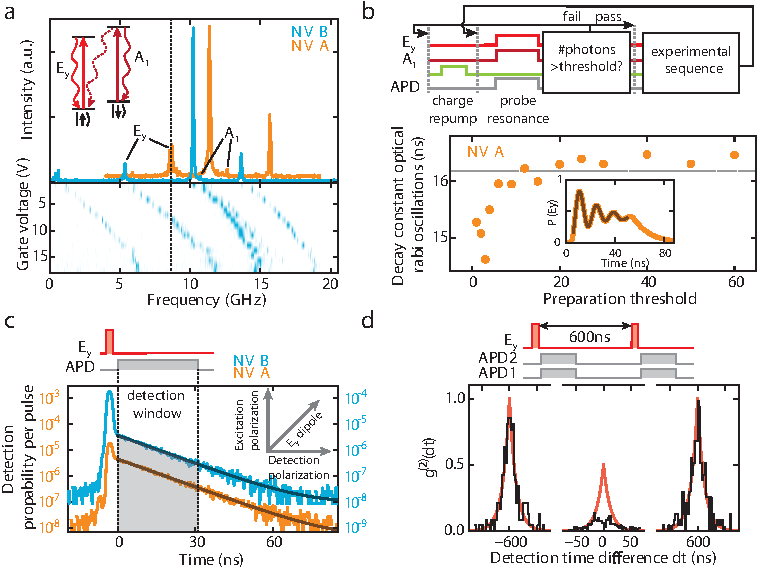
\includegraphics{fig2_ind_photons}
	\caption{\label{fig:LDE-fig2} \textbf{Generating and detecting indistinguishable photons.}
	\textbf{a,} Excitation spectra; frequency relative to 470.4515$\,$THz. By applying a voltage to the gates of NV~B the $E_\text{y}$ transitions are tuned into resonance. 
	\textbf{b,} Dynamical preparation of charge and optical resonance. Top: Preparation protocol. A 10$\,\mu$s green laser pulse pumps the NV into its negative charge state~\cite{Robledo_Nature_2011}. The transition frequencies are probed by exciting the $E_\text{y}$ and $A_\text{1}$ transitions for 60$\,\mu$s. Conditional on surpassing a certain number of photons detected the experiment is started (pass) or preparation is repeated (fail). APD, avalanche photodiode. Bottom: Line-narrowing effect of the preparation shown by the dependence of the decay time of optical Rabi oscillations on preparation threshold. Dashed line indicates lifetime-limited damping~\cite{Robledo_Phys.Rev.Lett._2010}. 
	% For the entanglement experiment we choose a threshold of 45 (20) photons for NV~A (NV~B). 
	\textbf{c,} Resonant optical excitation and detection. The polarisation axis of the detection path is aligned perpendicular to the excitation axis. The dipole axis of the $E_\text{y}$ transition is oriented in between these two axes (inset). Remaining laser light reflection is time-filtered by defining a photon detection window that starts after the laser pulse. 
	\textbf{d,} Two-photon quantum interference using resonant excitation and detection. The $g^{(2)}$ correlation function is obtained from all coincidence detection events of APD~1 and APD~2 during the entanglement experiment (see Supporting Material). The side-peaks are fit to an exponential decay; from the fit values, we obtain the expected central peak shape $g_\perp^{(2)}$ (red line) for non-interfering photons. The visibility of the interference is given by $(g_\perp^{(2)}-g^{(2)})/g_\perp^{(2)}$.}
\end{figure}


Charge fluctuations near the NV centre also affect the optical frequencies. To counteract photo-ionisation we need to regularly apply a green laser pulse to re-pump the NV centre into the desired charge state. This re-pump pulse changes the local electrostatic environment, leading to jumps of several line-widths in the optical transition frequencies~\cite{Robledo_Phys.Rev.Lett._2010}. To overcome these effects, we only initiate an experiment if the number of photons collected during a two-laser probe stage (Fig.~\ref{fig:LDE-fig2}b) exceeds a threshold, thereby ensuring that the NV centre optical transitions are on resonance with the lasers (see chapter~\ref{sec:CR-verification}). The preparation procedure markedly improves the observed optical coherence: as the probe threshold is increased, optical Rabi oscillations persist for longer times (see Fig.~\ref{fig:LDE-fig2}b). For high thresholds, the optical damping time saturates around the value expected for a lifetime-limited line-width~\cite{Robledo_Phys.Rev.Lett._2010}, indicating that the effect of spectral jumps induced by the re-pump laser is strongly mitigated.

Besides photon indistinguishability, successful execution of the protocol also requires that the detection probability of resonantly emitted photons exceeds that of scattered laser photons and of detector dark counts. This is particularly demanding for NV centres since only about 3\% of their emission is in the zero-phonon line and useful for the protocol. To minimise detection of laser photons, we use both a cross-polarised excitation-detection scheme (Fig.~\ref{fig:LDE-fig2}c inset) and a detection time filter that exploits the difference between the length of the laser pulse (2$\,$ns) and the NV centre's excited state lifetime (12\,ns) (Fig.\,\ref{fig:LDE-fig2}c). For a typical detection window used, this reduces the contribution of scattered laser photons to about 1\%. Combined with micro-fabricated solid-immersion lenses for enhanced collection efficiency (Fig.~\ref{fig:LDE-fig1-setup}b) and spectral filtering for suppressing non-resonant NV emission, we obtain a detection probability of a resonant NV photon of about $4\times10^{-4}$ per pulse --- about 70 times higher than the sum of background contributions.

The degree of photon indistinguishability and background suppression can be obtained directly from the second-order autocorrelation function $g^{(2)}$, which we extract from our entanglement experiment (see Supporting Material). For fully distinguishable photons, the value of $g^{(2)}$ would reach 0.5 at zero arrival time difference. A strong deviation from this behaviour is observed (Fig.~\ref{fig:LDE-fig2}d) due to two-photon quantum interference~\cite{Hong_Phys.Rev.Lett._1987} that, for perfectly indistinguishable photons, would make the central peak fully vanish. The remaining coincidences are likely caused by (temperature-dependent) phonon-induced transitions between optically excited states~\cite{Fu_Phys.Rev.Lett._2009} in NV~A. The visibility of the two-photon interference observed here --- $(80\pm5)$\% for $|dt| < 2.56\,$ns --- is a significant improvement over previously measured values~\cite{Bernien_Phys.Rev.Lett._2012,Sipahigil_Phys.Rev.Lett._2012} and key to the success of the entangling scheme.

To experimentally generate and detect remote entanglement, we run the following sequence: First, both NV centres are independently prepared into the correct charge state and brought into optical resonance according to the scheme in figure~\ref{fig:LDE-fig2}b. Then we apply the entangling protocol shown in figure~\ref{fig:LDE-fig1-protocol} using a 600$\,$ns delay between the two optical excitation rounds. We repeat the protocol 300 times before we return to the resonance preparation step; this number is a compromise between maximising the attempt rate and minimising the probability of NV centre ionisation. A fast logic circuit monitors the photon counts in real time and triggers single-shot qubit readout on each setup whenever entanglement is heralded, i.e. whenever a single photon is detected in each round of the protocol. The readout projects each qubit onto the \{$\ket{\up}$, $\ket{\down}$\} states (Z-basis), or on the \{$\ket{\up} \pm \ket{\down}$, $\ket{\up} \mp \ket{\down}$\} states (X or $-$X basis). The latter two are achieved by first rotating the qubit by $\pi/2$ using a microwave pulse before readout. By correlating the resulting single-qubit readout outcomes we can verify the generation of the desired entangled states. To obtain reliable estimates of the two-qubit state probabilities, we correct the raw data with a maximum-likelihood method for local readout infidelities. These readout errors are known accurately from regular calibrations performed during the experiment (see Supporting Material).

\subsection{Demonstration of remote entanglement}

Figure~\ref{fig:LDE-fig3} shows the obtained correlations. When both qubits are measured along Z (readout basis \{Z,Z\}), the states $\psi^+$ and $\psi^-$ (as identified by their different photon signatures) display strongly anti-correlated readout results (odd parity). The coherence of the joint qubit state is revealed by measurements performed in rotated bases (\{X,X\}, \{$-$X,X\}), which also exhibit significant correlations. Furthermore, these measurements allow us to distinguish between states $\psi^+$ and $\psi^-$. For $\psi^+$ the \{X,X\} (\{$-$X,X\}), outcomes exhibit even (odd) parity, whereas the $\psi^-$ state displays the opposite behaviour, as expected. The observed parities demonstrate that the experiment yields the two desired entangled states.

\begin{figure}[tp]
	\centering
	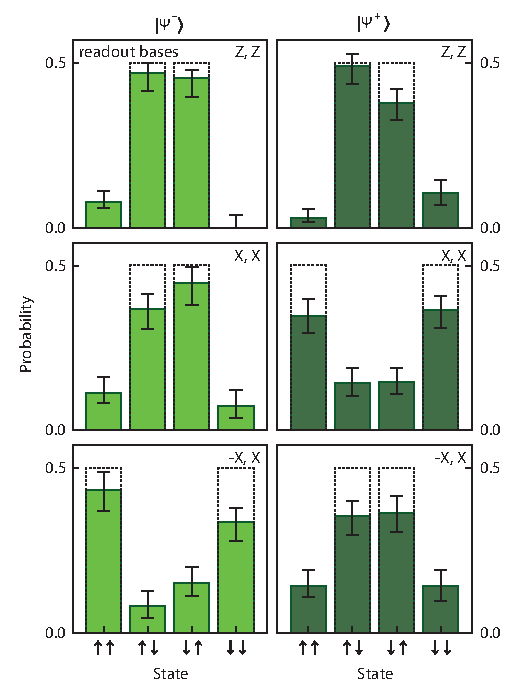
\includegraphics{H_Bernien_fig3}
	\caption{\label{fig:LDE-fig3} \textbf{Verification of entanglement by spin-spin correlations.} Each time that entanglement is heralded the spin qubits are individually read out and their results correlated. The readout bases for NV~A and NV~B can be rotated by individual microwave control (see text). The state probabilities are obtained by a maximum-likelihood estimation on the raw readout results (see Supporting Material). Error bars depict 68\% confidence intervals; dashed lines indicate expected results for perfect state fidelity. Data is obtained from 739 heralding events. For $\psi^-$, the detection window in each round is set to 38.4$\,$ns, and the maximum absolute detection time difference $|\delta\tau|$ between the two photons relative to their laser pulses is restricted to 25.6$\,$ns. $\delta\tau=\tau_2-\tau_1$, where $\tau_1$ is the arrival time of the first photon relative to the first laser pulse and $\tau_2$ the arrival time of the second photon relative to the second laser pulse. For $\psi^+$ the second detection window is set to 19.2$\,$ns with $|\delta\tau|<12.8\,$ns, in order to reduce the effect of photo-detector after-pulsing.}
\end{figure}

We calculate a strict lower bound on the state fidelity by combining the measurement results from different bases (see Supporting Material):
\begin{equation}\label{eq:LDE_LB}
F = \langle\psi^\pm|\rho|\psi^\pm \rangle \geq \ 1/2(P_{\uparrow\downarrow}+P_{\downarrow\uparrow}+C)-\sqrt{P_{\uparrow\uparrow}P_{\downarrow\downarrow}},
\end{equation}
where $P_{ij}$ is the probability for the measurement outcome $ij$ in the \{Z,Z\} basis (i.e. the diagonal elements of the density matrix $\rho$) and $C$ is the contrast between odd and even outcomes in the rotated bases. We find a lower bound of $(69\pm5)$\% for $\psi^-$ and $(58\pm6)$\% for $\psi^+$, and probabilities of 99.98\% and 91.8\%, respectively, that the state fidelity is above the classical limit of 0.5. These values firmly establish that we have created remote entanglement.

The lower bound on the state fidelity given above takes into account the possible presence of coherence within the even-parity subspace \{$\uu$, $\dd$\}. However, the protocol selects out states with odd parity and therefore this coherence is expected to be absent. To compare the results to the expected value and to account for sources of error, we set the related (square-root) term in Eq. 1 to zero and obtain for the data in figure~\ref{fig:LDE-fig3} as best estimate $F=(73\pm4)$\% for $\psi^-$ and $F=(64\pm5)\%$ for $\psi^+$.

Several known error sources contribute to the observed fidelity. Most importantly, imperfect photon indistinguishability reduces the coherence of the state. The fidelity is further decreased by errors in the microwave pulses (estimated at 3.5\%), spin initialisation (2\%), spin decoherence ($<1$\%) and spin flips during the optical excitation (1\%) (see Supporting Material). Moreover, $\psi^+$ is affected by after-pulsing, whereby detection of a photon in the first round triggers a fake detector click in the second round. Such after-pulsing leads to a distortion of the correlations (see for example the increased probability for $\dd$ in figure~\ref{fig:LDE-fig3}) and thereby a reduction in fidelity for $\psi^+$ (see Supporting Material). Besides these errors that reduce the actual state fidelity, the measured value is also slightly lowered by a conservative estimation for readout infidelities and by errors in the final microwave $\pi/2$ pulse used for reading out in a rotated basis.

The success probability of the protocol is given by $P_\psi =1/2 \eta_\text{A}\eta_\text{B}$. $\eta_i$ is the overall detection efficiency of resonant photons from NV $i$ and the factor 1/2 takes into account cases where the two spins are projected into $\dd$ or $\uu$, which are filtered out by their different photon signature. In the current experiment we estimate $P_\psi \approx 1.6 10^{-7}$. The entanglement attempt rate is about 20$\,$kHz, yielding one entanglement event per 10 minutes. This is in good agreement with the 739 entanglement events obtained over a time of 158 hours.

Creation of entanglement between distant spin qubits in diamond, as reported here, opens the door to extending the remarkable properties of NV-based quantum registers towards applications in quantum information science. A natural path forward is the incorporation of auxiliary nuclear spin qubits at the local nodes. In the following we discuss a second experiment where the nitrogen spin initialization and decoherence protected gates (as described in chapter \ref{ch:AMC}) are combined with an improved entanglement protocol to realize a deterministic Bell-state measurement which enables teleportation between a single nuclear spin and a distant electron spin.

\section{Teleportation}

Teleportation allows quantum information to be faithfully transmitted over arbitrary distances provided the two parties (``Alice'' and ``Bob'') have previously established a shared entangled state and can communicate classically.
The teleportation protocol is sketched in Fig.~\ref{LDE:fig4}. At the start, Alice is in possession of the state to be teleported (qubit 1) which is most generally given by $\ket\psi = \alpha\ket0 + \beta\ket1$. Alice and Bob each have one qubit of an entangled pair (qubits 2 and 3) in the joint state $\ket{\Psi^-}_{23} = (\ket{01}_{23} - \ket{10}_{23})/\sqrt2$. The combined state of all three qubits can be rewritten as
\begin{align}
    \ket\psi_1 \otimes \ket{\Psi^-}_{23} = \frac{1}{2} \big( 
        & \ket{\Phi^+}_{12} \otimes (\alpha\ket1_3 - \beta\ket0_3) \nonumber\\
        + & \ket{\Phi^-}_{12} \otimes (\alpha\ket1_3 + \beta\ket0_3) \nonumber\\
        + & \ket{\Psi^+}_{12} \otimes (- \alpha\ket0_3 + \beta\ket1_3) \nonumber\\
        - & \ket{\Psi^-}_{12} \otimes (\alpha\ket0_3 + \beta\ket1_3)
        \big),
\end{align}
where $\ket{\Phi^\pm} = (\ket{00}\pm\ket{11})/\sqrt2$ and $\ket{\Psi^\pm} = (\ket{01}\pm\ket{10})/\sqrt2$ are the four Bell states. To teleport the quantum state Alice performs a joint measurement on her qubits (qubits 1 and 2) in the Bell basis, projecting Bob's qubit into a state that is equal to $\ket\psi$ up to a unitary operation that depends on the outcome of Alice's measurement. Alice sends the outcome via a classical communication channel to Bob, who can then recover the original state by applying the corresponding local transformation.

Because the source qubit state always disappears on Alice's side, it is irrevocably lost whenever the protocol fails. Therefore, to ensure that each qubit state inserted into the teleporter unconditionally re-appears on Bob's side, Alice must be able to distinguish between all four Bell states in a single shot and Bob has to preserve the coherence of the target qubit during the communication of the outcome and the final conditional transformation. Several pioneering experiments have explored teleportation between remote nodes~\cite{Olmschenk_Science_2009,Nolleke_Phys.Rev.Lett._2013,Krauter_NatPhys_2013} but unconditional teleportation between long-lived qubits~\cite{Awschalom_Science_2013,Devoret_Science_2013,Monroe_Science_2013} has so far only been demonstrated within a local qubit register~\cite{Riebe_Nature_2004,Barrett_Nature_2004,Steffen_Nature_2013}.

\begin{figure*}
    \centering
    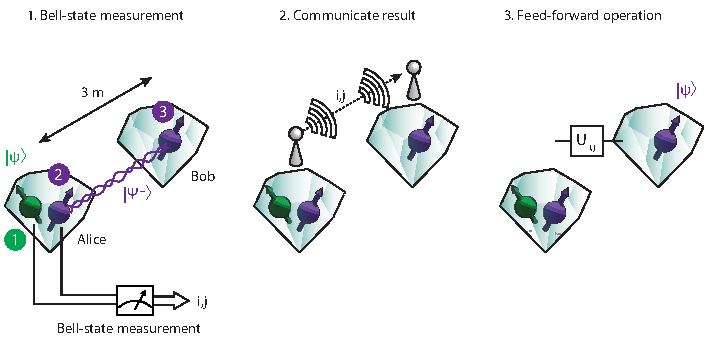
\includegraphics{fig4_teleportation_scheme}
    \caption{
    \label{LDE:fig4} 
    \textbf{Teleportation scheme.} 
    General scheme for teleportation. In our experiment Alice and Bob each control a single NV center in a single-crystal CVD-grown diamond by operating an independent cryogenic confocal microscope setup (T = 8\,K for Alice and T  = 4\,K for Bob). 
    % See supplementary methods for details.
    }
\end{figure*}

Here we demonstrate unconditional teleportation between diamond spin qubits residing in independent setups separated by 3 meters. We achieve this result by fully separating the generation of remote entanglement (the preparation of the teleporter) from the two-qubit Bell-state measurement and feed-forward (the actual teleportation action). In particular, a photonic channel is used to generate heralded remote entanglement between two nitrogen-vacancy (NV) center electronic spins, while the teleportation protocol solely exploits matter qubits that – unlike photonic qubits – allow for a deterministic Bell-state measurement with current technology. The source state is encoded in a nuclear spin close to one of the NV electron spins after preparation of the teleporter. We preserve the target qubit's coherence by dynamical decoupling while the measurement outcome is forwarded and the final correction pulse is applied. This protocol ensures that the source state is successfully teleported in each of the experimental runs.

In our experiment Alice and Bob each operate an independent low-temperature confocal microscope setup that addresses a single NV center. The two NV electronic spins (labeled as qubits 2 and 3) are used as the distributed entangled pair that is the medium for teleportation. These spins can be initialized and read out in a single shot by spin-resolved optical excitation~\cite{Robledo_Nature_2011} and coherently manipulated using microwave (MW) pulses~\cite{Lange_Science_2010}. 

To prepare the teleporter we initialize the electrons in the non-local entangled state $\ket{\Psi^-}_{23} = (\ket{01}_{23} - \ket{10}_{23})/\sqrt2$ through a recently demonstrated protocol~\cite{Barrett_Phys.Rev.A_2005,Bernien_Nature_2013} that is based on local entanglement between electron spin and photon number and subsequent joint measurement of the photons. Because successful entanglement generation is heralded by photon detection events, the protocol is robust against photon loss. Compared to the initial demonstration of this entangling protocol (~\ref{sec:HE}) we have further enhanced the efficiency of photon collection from our device through an anti-reflection coating. Also, we have significantly improved both the spectral stability of the NV center's optical transition and the charge state initialization by resonant re-pumping on the neutral-charge state zero-phonon line~\cite{Siyushev_Phys.Rev.Lett._2013}. As a result we were able to increase the generation rate of the entangled state $\ket{\Psi^-}_{23}$ fivefold to $1/250\, \mathrm s^{-1}$ and improve the entangled state fidelity from 0.73 to an estimated 0.87 (see below).

\begin{figure*}
	\centering
    \includegraphics{fig5_Prepare_teleporter}
    \caption{
    \label{fig:LDE-fig5} 
    \textbf{Preparation of the teleporter.}
    (a) Circuit diagram for the periodic measurement-based re-initialization of the nuclear spin (qubit 1) in between remote entanglement generation attempts. Both the probability for success per attempt and the time duration of a single attempt are indicated for the initialization by measurement of qubit 1 and the generation of entanglement between qubits 2 and 3. 
    (b) Measured probability P($\ket1$) to preserve the initialized nuclear spin state $\ket1$ as a function of number of entanglement generation attempts $N_\text{ent}$. A fit (solid line) to a rate-equation model yields a probability of $(0.85 \pm 0.05) \times 10^{-3}$ per entanglement generation attempt that the nuclear spin flips. The dashed line marks the maximum number of attempts before the nuclear spin is re-initialized ($N_\text{ent} = 250$). }
\end{figure*}



The additional qubit in Alice's node --- essential for making the teleportation unconditional --- is provided by the nitrogen-14 nuclear spin of Alice's NV (qubit 1). Before establishing the entanglement link, this nuclear spin is initialized into state $\ket1$ by a projective measurement via the electron spin~\cite{Robledo_Nature_2011}. We reinitialize the nuclear spin after each 250 entanglement attempts in order to preserve its purity (Figs.~\ref{fig:LDE-fig5}a,b). We prepare the source state after establishing remote entanglement, thus avoiding possible dephasing of the source state by repeated optical excitation of the nearby electron~\cite{Jiang_Phys.Rev.Lett._2008,Blok_NatPhys_2014} during entanglement generation. We employ a decoherence-protected gate~\cite{vanderSar_Nature_2012} on Alice's side to set the nuclear spin to the source state $\ket\psi = \alpha\ket0 + \beta\ket1$. This gate combines two nuclear spin rotations with a refocusing pulse on the electron spin such that the entangled state is efficiently preserved for the duration of the gate (Figs.~\ref{fig:LDE-fig6}a). This operation concludes the preparation of the teleporter and the insertion of the source qubit, with the three-qubit system left in the state $\ket\psi_1 \otimes \ket{\Psi^-}_{23} = (\alpha\ket0_1 + \beta\ket1_1) \otimes (\ket{01}_{23} - \ket{10}_{23})/\sqrt2$.

\begin{figure*}
	\centering
    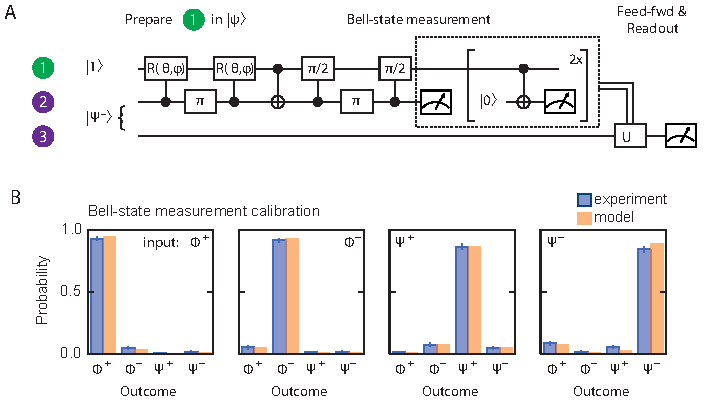
\includegraphics{fig6_circuit_diagram_bell_state_measurement}
    \caption{
    \label{fig:LDE-fig6} 
    \textbf{Deterministic Bell-state measurement (BSM) and real-time feed-forward.}
    (a) Circuit diagram of our implementation. The label `e' (`N') indicates operations acting on the electron spin (nitrogen nuclear spin). To enhance the readout fidelity for the nuclear spin, we perform the mapping to the electron spin via a CNOT and the subsequent electron readout twice. While Alice is performing her BSM Bob applies an XY4 decoupling sequence on his electron qubit. After receiving the BSM outcome from Alice, Bob applies the feed-forward operation $U$ and reads out his qubit. $\pi_{x,y}$ denote rotations around the $x$-axis and $y$-axis, respectively. 
    (b) Calibration of the BSM by inserting the four different Bell states on Alice's side and determining the probability with which the ideal outcome is observed (blue bars). Data is not corrected for imperfect preparation of the input states. Expectations based on independently determined experimental imperfections are shown in orange. Error bars are two statistical s.d.
    }
\end{figure*}


At the heart of unconditional qubit teleportation is a deterministic Bell-state measurement (BSM) by Alice on qubits 1 and 2 that generally involves two steps. First, the four Bell states are mapped onto the four different qubit eigenstates $\ket{i}_1 \ket{j}_2$ by quantum gate operations. In the second step each of the two qubits is read out in a single shot and the two measurement outcomes are sent to Bob. Our implementation of this scheme is shown in Figs.~\ref{fig:LDE-fig6}a. We implement the Bell-state mapping by applying a two-qubit controlled-NOT gate (CNOT) followed by a $\pi/2$ rotation on the nuclear spin using another decoherence-protected gate. Then we read out the electron spin in a single shot (average fidelity $0.963\pm0.005$). Finally we read out the nuclear spin by mapping its state onto the electron spin followed by electron spin readout. The two single-shot readout results give the outcome of the BSM.

We benchmark the BSM by preparing each of the four Bell states as input states in Alice's register (Fig.~\ref{fig:LDE-fig6}b). This procedure yields an uncorrected mean fidelity, given by the probability to obtain the measurement result corresponding to the prepared Bell state, of $0.89\pm0.02$. To gain more insight into the sources of imperfections we compare the data with numerical simulations that use the independently determined infidelities of the nuclear spin initialization, CNOT gate, and electron single-shot readout as input. These simulations predict an average fidelity of 0.9 (Fig.~\ref{fig:LDE-fig6}b), in excellent agreement with the data. Taking known errors in the preparation of the input states into account, we infer a BSM fidelity of $0.93\pm0.02$.

The final challenge for successful unconditional teleportation is to maintain the coherence of Bob's target qubit (qubit 3) during the BSM and feed-forward. In our experiment, Bob's qubit is mostly affected by interactions with the surrounding nuclear spin bath. We counteract this decoherence by applying an XY4 dynamical decoupling sequence~\cite{Lange_Science_2010}. The time between entanglement generation and the triggering of the feed-forward operation based on the BSM outcome is 300\,\textmicro s. For this duration the decoupling protocol preserves the qubit state with an average fidelity of $0.96\pm0.02$.

We first verify that the teleporter is calibrated correctly by applying it to the nominal input state $\ket Y = (\ket0+\ii\ket1)/\sqrt2$ and performing tomography on the state that appears on Bob's side. The reconstructed density matrix (Fig.~\ref{fig:LDE-fig7}B) shows that the target state vector is aligned well with $Y$ and therefore that the reference frames of Alice and Bob are correctly set.

\begin{figure*}
	\centering
    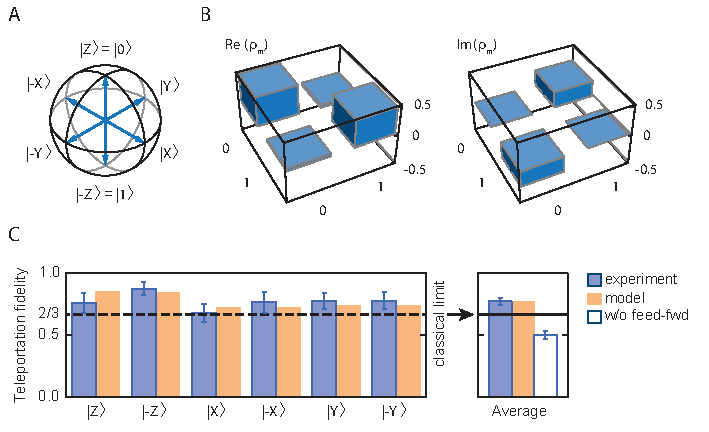
\includegraphics{fig7_teleportation_data}
    \caption {
    \label{fig:LDE-fig7} 
    \textbf{Demonstration of unconditional quantum teleportation between remote qubits.}
    (a) Bloch sphere with the six mutually unbiased basis states that we teleport. $\ket{\pm X} = (\ket0 \pm \ket1)/\sqrt2$, $\ket{\pm Y} = (\ket0 \pm \ii \ket1)/\sqrt2$.
    (b) State tomography after teleportation of the input state $\ket Y$. We determine the density matrix $\rho_\mathrm m$ by measuring the expectation values of the Pauli spin operators, $\langle \sigma_x \rangle$, $\langle \sigma_y \rangle$, $\langle \sigma_z \rangle$, where the required qubit rotations before readout are performed conditional on the BSM outcome. The measured (ideal) entries of the density matrix are $\rho_{00} = 1 - \rho_{11} = 0.52 \pm 0.08 \; (0.5)$ and $\rho_{01} = \rho_{10}^* = 0.05 \pm 0.08 - \ii 0.28 \pm \ii 0.07\; (- \ii 0.5)$, respectively.
    (c) Average teleportation fidelity from the measured fidelities of the six states (blue bars). Sample sizes are (left to right) 54, 89, 73, 49, 52, and 47. Predictions from simulations are shown in orange. Without feed-forward, the target state is completely mixed (white bar). The horizontal line marks the classical limit of $2/3$. Data is not corrected for source state initialization errors. Uncertainties are one statistical s.d. 
    }
\end{figure*}
To prove that our quantum teleporter outperforms any classical communication strategy, we teleport an unbiased set of six basis states $\ket\psi$ (Fig.~\ref{fig:LDE-fig7}A) and determine the fidelity of the teleported state on Bob's side with respect to the ideal input state. In these experiments we use a feed-forward operation that maps the ideal state of qubit 3 onto a qubit eigenstate such that the readout directly yields the teleportation fidelity. Since the feed-forward operation is conditional on the BSM outcome, ignoring the BSM outcome yields a completely mixed state and random outcomes ensuring that no information is transmitted. Without feed-forward we indeed observe an average teleportation fidelity of $\langle F \rangle = 0.50 \pm 0.03$ (Fig.~\ref{fig:LDE-fig7}C). In contrast, including the feed-forward loop we find $\langle F \rangle = 0.77 \pm 0.03$. This value exceeds the classical limit of $2/3$ by more than 3 standard deviations, thus proving the quantum nature of our teleporter. We note that this fidelity presents a lower bound on the actual teleportation fidelity because it does not take into account initialization errors of the source state. Importantly, this result is obtained without any post-selection: each teleportation attempt is included in the data presented here.

We also simulate the outcomes by using independently determined infidelities in the protocol. The only unknown parameter is the fidelity of the entangled state shared by Alice and Bob. We find that our data is well reproduced by the simulations if we assume a fidelity to the ideal Bell state $\ket{\Psi^-}_{23}$ of 0.87 (Fig.~\ref{fig:LDE-fig7}C). The simulations also enable us to quantify the effect of imperfect initialization of the source qubit on the measured fidelities. In this way we estimate the teleportation fidelity to be $\sim 0.86$.

The ability to generate remote entanglement and to control and read out multiple qubits per node as shown in the present teleportation experiment makes NV centers a leading candidate for realizing a quantum network. Our teleportation scheme is both unconditional and scalable to large distances as it can mitigate photon loss by heralding and purification of the distributed entangled state~\cite{Briegel_Phys.Rev.Lett._1998}. In future experiments we aim to supplement our current capabilities with quantum memories that are robust against optical excitation of the electrons, enabling remote entanglement purification and the connection of multiple nodes into the network. A promising route is the use of weakly coupled nuclear spins~\cite{Taminiau_Phys.Rev.Lett._2012,Kolkowitz_Phys.Rev.Lett._2012,Zhao_NatNano_2012} on which multi-qubit quantum control has very recently been demonstrated~\cite{Taminiau_NatNano_2014}. For such nuclear spins, coherence times of over 1 second under optical excitation have been reported~\cite{Maurer_Science_2012}, while the incorporation of NV centers into optical cavities may enable remote entanglement generation on millisecond timescales~\cite{Loncar_MRS_2013}. Furthermore, the entanglement and readout fidelities reported here are sufficient for a violation of a Bell inequality with the detection loophole closed, making NV centers a promising system for realizing a loophole-free Bell test and device-independent quantum key distribution~\cite{Brunner_Rev.Mod.Phys._2014}. 




\clearpage

\bibliographystyle{../thesis}
\bibliography{lde}

%\include{ch_teleportation/teleportation}
%\include{ch_outlook/outlook}

\backmatter
%\include{ch_at_the_end/summary}
%\include{ch_at_the_end/acknowledgements}
%\include{ch_at_the_end/publications}
%\include{ch_at_the_end/cv}
%
\end{document}
